\chapter{Grundlagen}
\label{ch: Grundlagen}
	Für ein besseres Verständnis, der in Kapitel \ref{ch: Konzeptionierung} angewandten Methoden, werden anbei die Grundlagen behandelt. Informationen zu der verwendeten Hard- und Software wurden bereits in der vorangegangenen Bachelorarbeit vermittelt. Die in Kapitel \ref{ch: Grundlagen} erwähnte Personenerkennung ist eine Abwandlung der Objekterkennung. Im Folgenden werden sowohl herkömmliche als auch state-of-the-art Lösungen zur Objekterkennung präsentiert. Letzteres beinhaltet unter anderem das Gebiet der neuronalen Netzwerke. Somit werden zunächst die neuronalen Netze und ihre Eigenschaften besprochen, bevor die Grundlagen der Objekterkennung erläutert werden. 
 
	
 	\section{Neuronale Netze}
	\label{sec: ROS}
	
	Das Neuronennetz des menschlichen Gehirns dient als Vorbild für künstliche, neuronale Netze (KNN) \cite{neuronennetz}. KNNs werden heutzutage verwendet, um diverse Anwendungsprobleme zu lösen.
	Sie ermöglichen es komplexe Strukturen und Muster aus großen Datenmengen zu erkennen.
	\cite{neuronennetz}. Das in diesem Projekt zugrundeliegende Bildverarbeitungsproblem besitzt jene Eigenschaften und eignet sich für den Einsatz eines neuronalen Netzes als Problemlösung. Anders als bei regelbasierten Systemen verhalten sich KNNs grundlegend verschieden \cite{proba}. Sie lernen Verhaltensmuster basierend auf den entsprechenden Trainingsdaten \cite{proba}. Dies führt unter Umständen zu unvorhersehbaren Ergebnissen. Am vorliegenden, autonomen Logistikfahrzeug werden zur Personenerkennung derartige neuronale Netze untersucht.
	
		\subsection{Eigenschaften von neuronalen Netzen}
		\label{subsec: Eigenschaften von neuronalen Netzen}
		Die Grundlage für die Eingabe in ein neuronales Netz sind entsprechende, zu analysierende Daten. Bei einem Anwendungsfall, in dem eine Audiospur analysiert werden soll, können beispielsweise Frequenzspektren eingegeben werden. Ein klassisches Bildverarbeitungsproblem arbeitet mit den Pixeln eines Bildes. Hierbei werden Daten über eine Eingabeschicht in die darin enthaltenen Neuronen gegeben. \\
		
		\begin{figure}[H]
			\centering
			
			\begin{tikzpicture}[
				init/.style={
					draw,
					scale=1.5,
					circle,
					inner sep=2pt,
					font=\Huge,
					join = by -latex
				},
				squa/.style={
					draw,
					inner sep=2pt,
					font=\Large,
					join = by -latex
				},
				start chain=2,node distance=13mm
				]
				\node[on chain=2] 
				(x2) {\text{ }\text{ }$x_{j+1}$};
				\node[on chain=2,join=by o-latex] 
				{$w_{j+1}$};
				\node[on chain=2,init] (sigma) 
				{$\displaystyle\Sigma$};
				\node[on chain=2,squa,label=above:{\parbox{2cm}{\centering Aktivierungs-funktion}}] 
				{$f$};
				\node[on chain=2,label=above:Ausgabe,join=by -latex] 
				{$y$};
				\draw[fill=black](1,-0.425)circle(1pt);
				\draw[fill=black](1,-0.75)circle(1pt);
				\draw[fill=black](1,-1.075)circle(1pt);
				\begin{scope}[start chain=1]
					\node[on chain=1] at (0,1.5cm) 
					(x1) {$x_{j}$};
					\node[on chain=1,join=by o-latex] 
					(w1) {$w_{j}$};
				\end{scope}
				\begin{scope}[start chain=3]
					\node[on chain=3] at (0,-1.5cm) 
					(x3) {$x_{n}$};
					\node[on chain=3,label=below:Gewichte,join=by o-latex] 
					(w3) {$w_{n}$};
				\end{scope}
				%\node[label=above:\parbox{2cm}{\centering Bias \\ $b$}] at (sigma|-w1) (b) {};
				
				\draw[-latex] (w1) -- (sigma);
				\draw[-latex] (w3) -- (sigma);
				%\draw[o-latex] (b) -- (sigma);
				
				\draw[decorate,decoration={brace,mirror}] (x1.north west) -- node[left=10pt] {Eingabe} (x3.south west);
			\end{tikzpicture}
		
			\caption{Darstellung der prinzipiellen Funktion eines Neurons in einem neuronalen Netz. Drei aufeinander folgende Punkte deuten eine Fortsetzung an. \cite{neuron}}
			\label{fig: neuron}
		\end{figure}
		
		Der grundlegende Aufbau eines neuronalen Netzes besteht aus verschiedenen, miteinander verbundenen Schichten \cite{bildv2020}. Ein Neuron $i$ einer Schicht ist jeweils mit dem Neuron $j$ der folgenden Schicht über das Gewicht $w_{ij}$ verbunden \cite{bildv2020}. Die typische Struktur eines Neurons ist Abbildung \ref{fig: neuron} zu sehen.\\
		
		\begin{equation}
			s=\sum_{j=1}^n w_{ij}x_j
			\label{eq: Gewichtete Summe}
		\end{equation}
		\\
		
		 Es verarbeitet im Wesentlichen eingehende Bildinformationen $x_n$ und gibt diese durch die Ausgabe $y$ aus. Genauer wird mit den eingehenden Zahlenwerten eine gewichtete Summe $s$ gebildet. Diese wird dann auf eine Aktivierungsfunktion angewendet und ausgegeben \cite{bildv2020}. Diese aktiviert bzw. reizt das Neuron ab einem Schwellwert \cite{Kriesel}. Es gibt verschiedene Varianten der Aktivierungsfunktion, die je nach Netzarchitektur zur Anwendung kommen können. Gleichung \ref{eq: Gewichtete Summe} zeigt das mathematische Modell der gewichteten Summe $s$.\\
		
		
				
		\tikzset{%
			every neuron/.style={
				circle,
				draw,
				minimum size=1cm
			},
			neuron missing/.style={
				draw=none, 
				%scale=4,
				%rotate=90,
				%yshift=1,
				%text height=0.333cm,
				%execute at begin node=\color{black}$\cdots$
			},
		}
		\begin{figure}[H]
			\centering
			
			
			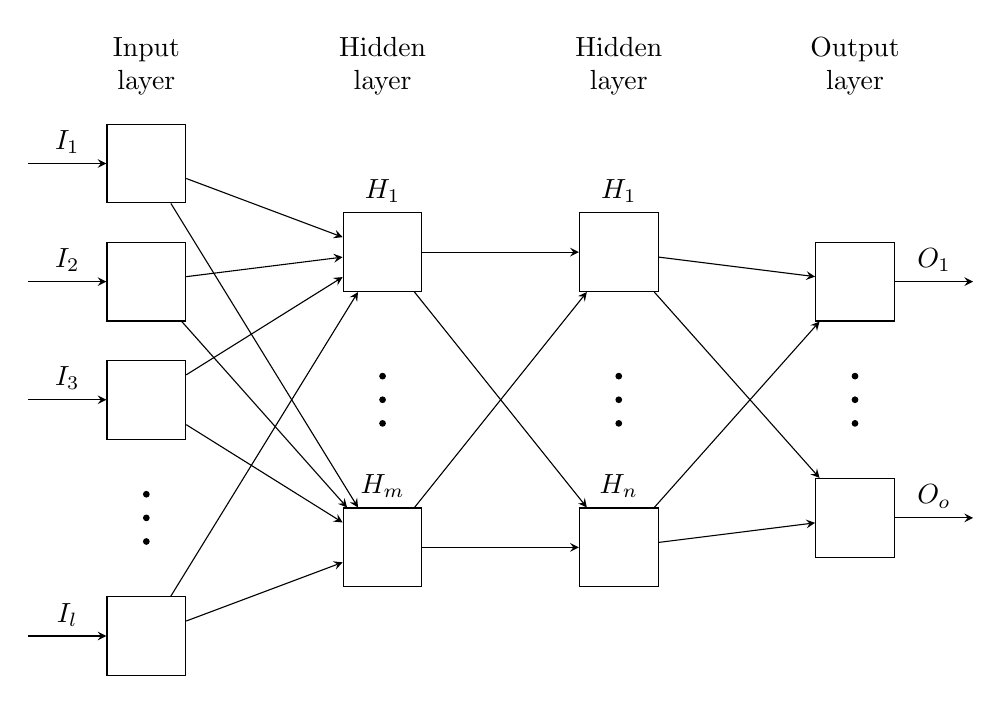
\begin{tikzpicture}[x=1.5cm, y=1.5cm, >=stealth]
				
				\foreach \m/\l [count=\y] in {1,2,3,missing,4}
				\node [every neuron/.try, neuron \m/.try] (input-\m) at (0,2.5-\y) {};
				
				\foreach \m [count=\y] in {1,missing,2}
				\node [every neuron/.try, neuron \m/.try ] (hidden1-\m) at (2,2-\y*1.25) {};
				
				\foreach \m [count=\y] in {1,missing,2}
				\node [every neuron/.try, neuron \m/.try ] (hidden1-\m) at (2,2-\y*1.25) {};
				
				\foreach \m [count=\y] in {1,missing,2}
				\node [every neuron/.try, neuron \m/.try ] (hidden2-\m) at (4,2-\y*1.25) {};
				
				\foreach \m [count=\y] in {1,missing,2}
				\node [every neuron/.try, neuron \m/.try ] (output-\m) at (6,1.5-\y) {};
				
				\foreach \l [count=\i] in {1,2,3,l}
				\draw [<-] (input-\i) -- ++(-1,0)
				node [above, midway] {$I_\l$};
				
				\foreach \l [count=\i] in {1,m}
				\node [above] at (hidden1-\i.north) {$H_\l$};
				
				\foreach \l [count=\i] in {1,n}
				\node [above] at (hidden2-\i.north) {$H_\l$};
				
				\foreach \l [count=\i] in {1,o}
				\draw [->] (output-\i) -- ++(1,0)
				node [above, midway] {$O_\l$};
				
				\foreach \i in {1,...,4}
				\foreach \j in {1,...,2}
				\draw [->] (input-\i) -- (hidden1-\j);
				
				\foreach \i in {1,...,2}
				\foreach \j in {1,...,2}
				\draw [->] (hidden1-\i) -- (hidden2-\j);
				
				\foreach \i in {1,...,2}
				\foreach \j in {1,...,2}
				\draw [->] (hidden2-\i) -- (output-\j);
				
				\foreach \l [count=\x from 0] in {Input, Hidden, Hidden, Output}
				\node [align=center, above] at (\x*2,2) {\l \\ layer};
				
				\draw[fill=black](0,-1.3)circle(1pt);
				\draw[fill=black](0,-1.5)circle(1pt);
				\draw[fill=black](0,-1.7)circle(1pt);
				\draw[fill=black](2,-0.3)circle(1pt);
				\draw[fill=black](2,-0.5)circle(1pt);
				\draw[fill=black](2,-0.7)circle(1pt);
				\draw[fill=black](4,-0.3)circle(1pt);
				\draw[fill=black](4,-0.5)circle(1pt);
				\draw[fill=black](4,-0.7)circle(1pt);
				\draw[fill=black](6,-0.3)circle(1pt);
				\draw[fill=black](6,-0.5)circle(1pt);
				\draw[fill=black](6,-0.7)circle(1pt);
				\end{tikzpicture}
				\caption{Prinzipielle Darstellung eines künstlichen, neuronalen Netzwerks. Neuronen werden als Kreise dargestellt. Drei aufeinander folgende Punkte deuten eine Fortsetzung an. Adaptiert aus \cite{neuron}.}
				\label{fig: neuronales netz }
		\end{figure}
	
		
		In Abbildung \ref{fig: neuronales netz } ist die Grundstruktur eines neuronalen Netzes veranschaulicht. Neuronen sind hier mit Kreisen angedeutet und bilden einzelne Schichten in den beispielhaft vertikal dargestellten Formationen. Hierbei wird zwischen Eingabe-, Zwischen- und Ausgabeschichten unterschieden. Entsprechende Neuronen sind mit $I$, $H$ und $O$ bezeichnet. Die Eingabeschicht nimmt Informationen in Form von Daten auf und gibt diese an die erste Zwischenschicht weiter. Die Anzahl der Zwischenschichten, oder auch verdeckte Schichten, ist in der Anwendung neuronaler Netze variabel. Am rechten Bildrand ist die Ausgabeschicht gezeigt, die die entsprechende Ausgabe des Netzes generiert.  
	
		\subsection{Lernprozess}
		Der Lernprozess von neuronalen Netzen zielt darauf ab, einer Netzstruktur ein gewünschtes Verhalten beizubringen \cite{proba}. Genauer sollen die in Abschnitt \ref{subsec: Eigenschaften von neuronalen Netzen} beschriebenen Gewichte so modifiziert werden, dass sie eine bestimmte Ausgabe erzeugen.\\
		
		Es wird zwischen drei wesentlichen Lernverfahren unterschieden, dem unüberwachten, dem bestärkenden und dem überwachten Lernen \cite{Kriesel}. Beim unüberwachten Lernen erkennt das Netz selbst Muster und versucht diese aus der eingegebenen Menge in Klassen zu unterteilen \cite{Kriesel}. Anders als beim unüberwachten Lernen lernt das Netz beim bestärkten Lernen mit einer Rückmeldung. Diese enthält Informationen darüber, ob ein errechnetes Ergebnis einer Trainingseinheit richtig oder falsch ist \cite{Kriesel}. Das überwachte Lernen setzt eine Trainingsmenge voraus, die neben der Eingabedaten auch das dazugehörige korrekte Ergebnis enthält \cite{Kriesel,bildv2020}. Im Falle einer Personenerkennung wäre beispielsweise ein Datensatz aus Bildern von Personen eine geeignete Trainingsmenge. In der sogenannten Vorwärtspropagierung wird durch eine Eingabe eine entsprechende Ausgabe erzeugt und diese mit dem korrekten Ergebnis verglichen \cite{bildv2020}. Ausgehend von einem KNN mit lediglich einer Schicht, werden die Gewichte dann mithilfe des aus dem vorangegangenen Vergleich entstandenen Fehlers korrigiert \cite{bildv2020}.\\
		
		Die meist genutzte Form des überwachten Lernens ist die Rückwärtspropagierung (engl. Backpropagation) oder Fehlerrückführung genannt \cite{Ertel}. Wie bereits beschrieben bestehen neuronale Netze häufig aus mehreren verdeckten Schichten. Für diese liegt beim Training jedoch kein Korrekturwert vor \cite{bildv2020}. Der Algorithmus der Rückwärtspropagierung ist eine mögliche Lösung dieses Problems. Die mathematische Grundlage für dieses Lernverfahren sind Gradientenabstiegsverfahren \cite{Kriesel,bildv2020}. Nach der Vorwärtspropagierung wird die Ausgabe des Netzes mit Sollwerten verglichen \cite{bildv2020}. Beim darauffolgenden Rückwärtsschritt wird durch die Fehlerrückführung für jede verdeckte Schicht ein Korrekturwert errechnet \cite{bildv2020}. Auch in dieser Masterarbeit werden Netze mithilfe der Rückwärtspropagierung trainiert und in diesem Kapitel \ref{ch: Verifikation} genauer erläutert.\\
		
	
		
		\subsection{Evaluation neuronaler Netze}
		\label{subsec: evaluation neuronaler netze}
		Es bestehen diverse Metriken für Objekterkennungssysteme, die derartige Systeme messbar machen. Im Rahmen dieser Masterarbeit wird zur Evaluation die Metrik \textit{Precision} und \textit{Recall} eingesetzt. Außerdem werden die neuronalen Netze anhand des Top-x Fehlers sowie der \textit{mean average precision} (mAP) verglichen. Die Grundlagen der entsprechenden Metriken werden im Folgenden vermittelt.\\
		
		\newcolumntype{C}[1]{>{\centering\arraybackslash}p{#1}}
\newcolumntype{M}[1]{>{\centering\arraybackslash}m{#1}}
\begin{table}[H]
	\caption{Tabelle zum besseren Verständnis der Begriffe \textit{True Positive}, \textit{False Positive}, \textit{False Negative} und \textit{True Negative}. In der jeweiligen Zelle wird ein Beispiel im praktischen Kontext der Personenerkennung genannt.}
	\begin{center}
		\begin{tabular}{|c|c|c|c|}
			\hline
			\multicolumn{2}{|c|}{\multirow{2}{*}{}}&\multicolumn{2}{c|}{Realität}\\ \cline{3-4}
			\multicolumn{2}{|c|}{}&Wahr&Falsch\\
			\hline
			\multirow{3.2}{*}{Ausgabe}&Wahr&\makecell{\textit{True Positive} (TP)\\ Realität: Person vorhanden\\ Ausgabe: Person vorhanden}& \makecell{\textit{False Positive} (FP) \\ Realität: Keine Person  \\ Ausgabe: Person vorhanden}\\ \cline{2-4}
			&Falsch&\makecell{\textit{False Negative} (FN)\\ Realität: Person vorhanden\\ Ausgabe: Keine Person}&\makecell{\textit{True Negative} (TN)\\ Realität: Keine Person\\ Ausgabe: Keine Person}\\
			\hline
		\end{tabular}
	\end{center}

	\label{fig: pr}
\end{table}
		
		\textit{Precision} und \textit{Recall} ist ein traditionelles Werkzeug zur Evaluation und Leistungsmessung \cite{precisionandrecall}. In Tabelle \ref{fig: pr} werden zum besseren Verständnis die Begrifflichkeiten \textit{True Positive} (TP), \textit{False Positive}(FP), \textit{False Negative} (FN) und \textit{True Negative} (TN) näher erläutert. Der \textit{Recall}-Wert $r(t)$ beschreibt die Fähigkeit eines Systems, tatsächlich positive Stichproben zu erkennen. Angewandt auf die Personenerkennung sind Bilder, auf denen Personen zu sehen sind, als tatsächlich positive Stichproben einzustufen. In Gleichung \ref{eq: recall} wird der \textit{Recall}-Wert durch eine Division von allen wahren positiven Werten $TP(t)$ und die Anzahl aller tatsächlich positiven Werte $n_{pos}$ berechnet. Die Variable $t$ definiert den eingestellten Schwellwert. Im Sachkontext ist der Wert als Konfidenz zu betrachten, bei der eine Person als solche klassifiziert wird. Für die Anwendung dieser Methode ist die Kenntnis über negative Beispiele der Stichprobe nicht notwendig \cite{bildundobjekt}.\\ 
		
		\begin{equation}
		r(t)=\frac{TP(t)}{TP(t)+FN(t)}
		\label{eq: recall}
		\end{equation}\\
		
		Der \textit{Precision}-Wert $p(t)$ berechnet sich durch das Verhältnis von allen wahren positiven Werten $TP(t)$, zu allen als positiv bewerteten Beispielen $TP(t)$ und $FP(t)$. Gleichung \ref{eq: precision} zeigt die entsprechende Berechnung. Durch diesen Wert wird verdeutlicht, wie gut ein System in der Lage ist tatsächlich wahre Werte von tatsächlich falschen Werten zu unterscheiden.\\
		
		\begin{equation}
		p(t)=\frac{TP(t)}{TP(t)+FP(t)}
		\label{eq: precision}
		\end{equation}\\
		
		Häufig muss in der Praxis ein Kompromiss zwischen \textit{Precision} und \textit{Recall} gefunden werden. Dies lässt sich anhand eines Beispiels in der Personenerkennung veranschaulichen. Das System zur Erkennung wird beispielhaft mit einem hohen \textit{Precision}- und einen niedrigen \textit{Recall}-Wert betrieben. Dies führt dazu, dass irrelevanter Bildinhalt selten als Person klassifiziert wird. Jedoch kommt es häufiger vor, dass keine Person detektiert wird, obwohl eine zu sehen ist. Legt man den Fokus auf einen hohen \textit{Recall}- und einen niedrigen \textit{Precision}-Wert würden Personen dann häufiger als Person klassifiziert werden. Jedoch wird irrelevanter Bildinhalt ebenfalls häufig als Person klassifiziert. Je nach Anwendungsfall eines Netzes wird dann der entsprechende Betriebspunkt zwischen \textit{Precision} und \textit{Recall} gewählt.\\
		
		Objekterkennungssysteme geben erkannte Objekt mithilfe eines Begrenzungsrahmens aus. Dieser wird mithilfe von Pixelkoordinaten passend zum untersuchten Bild angegeben. Der \textit{Intersection over Union} (IoU) Wert sagt aus, ob die Lokalisierung eines Objekts in einem Bild entsprechend genau ist. Als Grundlage dient hierfür ein Testdatensatz mit verschiedenen Bildern und grundwahren Begrenzungsrahmen für enthaltene Objekte. Zur Ermittlung des \textit{IoU}-Werts werden von einem Objekterkennungssystem ausgegebene mit grundwahren Begrenzungsrahmen verglichen. Hierbei lässt sich die überlappende und die zusammengesetzte Fläche beider Rahmen im Verhältnis setzen. Das Ergebnis ist der \textit{IoU}-Wert.    \\
		
		\begin{equation}
		mAP = \frac{1}{K}\sum_{i=1}^{K}\int_{0}^{1}p_i(r_i)dr
		\label{eq: map}
		\end{equation}\\
		
		Der \textit{mAP}-Wert oder auch die mittlere durchschnittliche Genauigkeit ist ein Indiz dafür, wie genau die Objekterkennung klassenübergreifend arbeitet. Die Berechnung dieses Wertes beinhaltet hierbei die bereits vorgestellten \textit{Precision} und \textit{Recall} Werte. Dieser Messwert ist besonders aussagekräftig, wenn Systeme lediglich eine Objektklasse erkennen können. Gleichung \ref{eq: map} zeigt die Berechnung der mittleren durchschnittlichen Genauigkeit. Die Variable $K$ ist die Menge aller Klassen, die durch das Netz erkannt werden können.  \\
		
		Eine einfache Betrachtung zur Evaluierung der Qualität hinsichtlich der Genauigkeit eines Netzes liefert der Top-$x$ Fehler. Der Platzhalter $x$ kann zunächst durch eine beliebige Zahl ersetzt werden. In der Praxis hat sich jedoch der Top-5 und der Top-1 Fehler als Vergleich durchgesetzt. Hierbei wird zunächst ein Bild durch ein beliebiges KNN analysiert und über die Ausgabeschicht extrahiert. Als Beispiel sollte sich im optimalen Fall die tatsächliche Klasse des Bildes unter den $x$ wahrscheinlichsten Klassen befinden, die über das Netz ausgegeben wurden. Folglich sagt der Top-1 Fehler aus, wie oft ein Netz ein eingegebenes Bild falsch klassifiziert hat. In vielen Paper zu neuen, künstlichen, neuronalen Netzen wird so die Genauigkeit mit bereits bestehenden Netzen verglichen.
		
		
		
		
		
		
	\section{Objekterkennung}
	\label{sec: Objekterkennung}
	Bei der visuellen Objekterkennung wird ein Objekt, das auf einem Bild gezeigt ist, mit einer gewissen Wahrscheinlichkeit inklusive der Position in der Abbildung erkannt. Die drei Abstraktionsebenen einer solchen Erkennung unterteilen sich in Bildklassifikation, Objektlokalisierung und semantische Segmentierung \cite{bildundobjekt}. Letzteres kommt in dieser Arbeit nicht zur Anwendung und wird aufgrund dessen im Folgenden nicht behandelt. Die Bildklassifikation beschreibt eine Zuweisung von Objektkategorien zu einem gegebenen Bild. Mithilfe einer Merkmalsextraktion werden Merkmalsvektoren extrahiert und können so in einem Klassifikator berechnet werden. In den folgenden Abschnitten wird auf die in dieser Arbeit eingesetzten Methoden zur Objekterkennung eingegangen. Hierbei werden insbesondere alternative Verfahren mit modernen state-of-the-art Lösungen zur Objekterkennung gegenübergestellt.  
	
	
		\subsection{Objekterkennung durch alternative Verfahren}
		\label{subsec: Objekterkennung durch alternative Verfahren}	
		
		
		Neben der neuronalen Netze gibt es weitere Methoden zur Objekterkennung. Ein gängiges Verfahren zur Merkmalsextraktion ist das sogenannte Histogram of oriented gradients (HoG) von \textit{Dalal} in Verbindung mit der \textit{Linear Support Vector Machine} (SVM).\\
		
		Bei diesem Verfahren wird ein Bild in kleine Bereiche, sogenannte Zellen, aufgeteilt \cite{hogsvm}. Für jede Zelle wird ein eindimensionales Histogram extrahiert \cite{hogsvm}. Dieses enthält Gradienten, die aus den Informationen der Pixel enstehen, wie zum Beispiel durch die Lichtintensität oder der Farbe. Hieraus lassen sich Kanten und Ecken und somit auch Konturen und Muster aus einem Bild erkennen. In den Abbildungen \ref{fiq: hog} a und b lässt sich die Umwandlung des \textit{HoGs} beobachten. Die Realität, so wie sie eine übliche Fotokamera widerspiegeln würde, ist in \ref{fiq: hog}a zu erkennen. Die entsprechenden Richtungen der Gradienten werden in \ref{fiq: hog}b dargestellt. \\
		
		
\begin{figure}[H]
	\centering
	\begin{minipage}[b]{0.45\textwidth}
		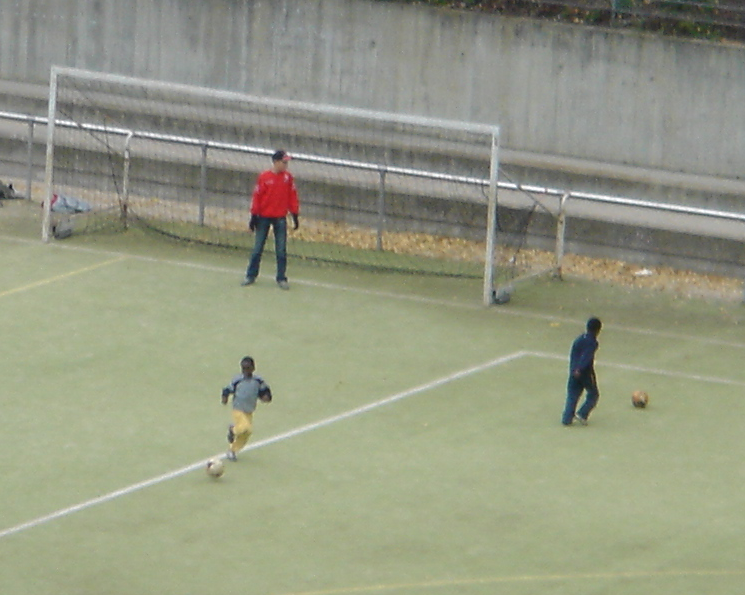
\includegraphics[width=\textwidth]{Bilder/hog1crop.png}
		\caption{(a)}
	\end{minipage}
	\hfill
	\begin{minipage}[b]{0.45\textwidth}
		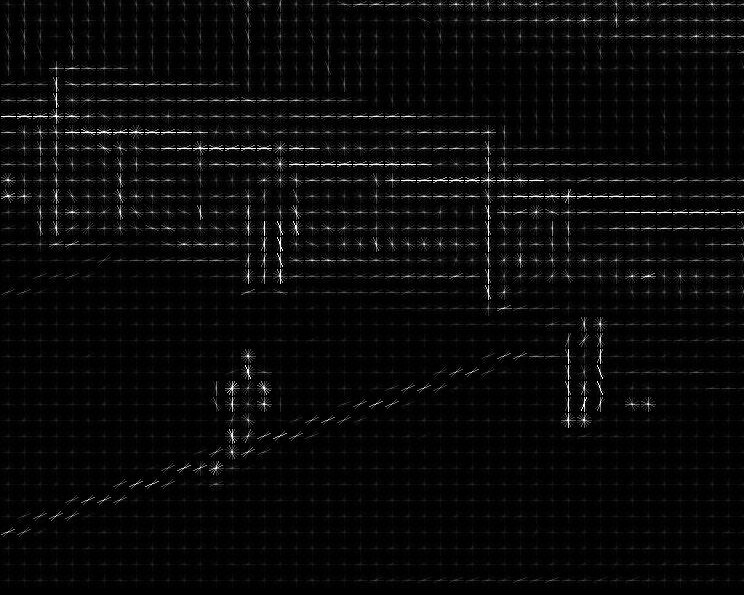
\includegraphics[width=\textwidth]{Bilder/hog2crop.jpg}
		\caption{(b)}
	\end{minipage}
	\caption{(a) Foto von drei spielenden Personen \cite{inria1}. (b) Darstellung der Gradienten, die durch einen HoG erzeugt worden sind. Die Analyse erfolgte mit Bild (a) \cite{inria1}.}
	\label{fiq: hog}
\end{figure}
		
		Die \textit{SVM} ist ein Funktionsapproximator für eine Objektklassifikation. Häufig wird dieser auf die Ausgangsdaten des \textit{HoGs} angewendet. Hierbei wird ein mathematisches Verfahren angewendet, das Klassen durch Trennungsebenen, sogenannte Hyperebenen, voneinander trennt. Wie auch bei den KNNs gibt es für \textit{SVMs} ein Lernprozess in Form des überwachten Lernens. Ziel der Algorithmen des Trainings einer \textit{SVM} ist es, die Hyperebenen so zu konstruieren, dass Objekte sicher klassifiziert werden können. In der Realität lassen sich Objekte rein mathematisch häufig nicht linear trennen. Nichtlineare Trennbarkeit bedeutet oft einen höheren Rechenaufwand. Somit verwendet die Methode der \textit{SVM} den sogenannten \textit{Kernel-Trick} \cite{svmalt}. Dieser transformiert Daten in eine höhere Dimension, um eine lineare Trennbarkeit zu erreichen \cite{svmalt}. Diese Methode hat sich vor allem aufgrund ihrer kurzen Rechenzeit durchgesetzt. In Abbildung \ref{fig: kerneltrick} a und b ist das Funktionsprinzip prinzipiell dargestellt. Darstellung \ref{fig: kerneltrick}a zeigt Objektklassen, die jeweils als Formen dargestellt sind. Eine lineare Trennbarkeit mittels einer Hyperebene ist in diesem Beispiel nicht möglich. Eine dritte Dimension wird in der Darstellung \ref{fig: kerneltrick}b verwendet, um die dargestellte, lineare Trennbarkeit zu erreichen.\\
		
			\begin{figure}[H]
			\begin{minipage}[b]{0.49\textwidth}
				(a)
				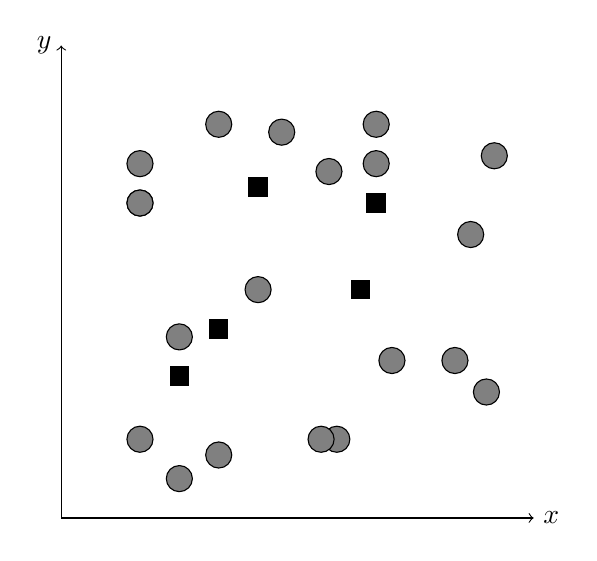
\begin{tikzpicture}
					\draw [->] (0,0,0) -- (6,0,0) node [at end, right] {$x$};
					\draw [->] (0,0,0) -- (0,6,0) node [at end, left] {$y$};
					\node [black,circle,draw,fill=gray](s) at (1,1,0){};
					\node [black,circle,draw,fill=gray](s) at (2,0.8,0){};
					\node [black,circle,draw,fill=gray](s) at (1.5,0.5,0){};
					\node [black,circle,draw,fill=gray](s) at (4,5,0){};
					\node [black,circle,draw,fill=gray](s) at (2,5,0){};
					\node [black,circle,draw,fill=gray](s) at (1,4.5,0){};
					\node [black,circle,draw,fill=gray](s) at (3.5,1,0){};
					\node [black,circle,draw,fill=gray](s) at (1,4,0){};
					\node [black,circle,draw,fill=gray](s) at (5.4,1.6,0){};
					\node [black,circle,draw,fill=gray](s) at (2.5,2.9,0){};
					\node [black,circle,draw,fill=gray](s) at (1.5,2.3,0){};
					\node [black,circle,draw,fill=gray](s) at (4.2,2,0){};
					\node [black,circle,draw,fill=gray](s) at (5,2,0){};
					\node [black,circle,draw,fill=gray](s) at (4,4.5,0){};
					\node [black,circle,draw,fill=gray](s) at (3.3,1,0){};
					\node [black,circle,draw,fill=gray](s) at (1,4,0){};
					\node [black,circle,draw,fill=gray](s) at (3.4,4.4,0){};
					\node [black,circle,draw,fill=gray](s) at (2.8,4.9,0){};
					\node [black,circle,draw,fill=gray](s) at (5.5,4.6,0){};
					\node [black,circle,draw,fill=gray](s) at (5.2,3.6,0){};
					
					\node [draw,fill=black](s) at (2,2.4,0){};
					\node [draw,fill=black](s) at (2.5,4.2,0){};
					\node [draw,fill=black](s) at (3.8,2.9,0){};
					\node [draw,fill=black](s) at (1.5,1.8,0){};
					\node [draw,fill=black](s) at (4,4,0){};
					
				\end{tikzpicture}
			\end{minipage}
			\begin{minipage}[b]{0.49\textwidth}
				(b)
				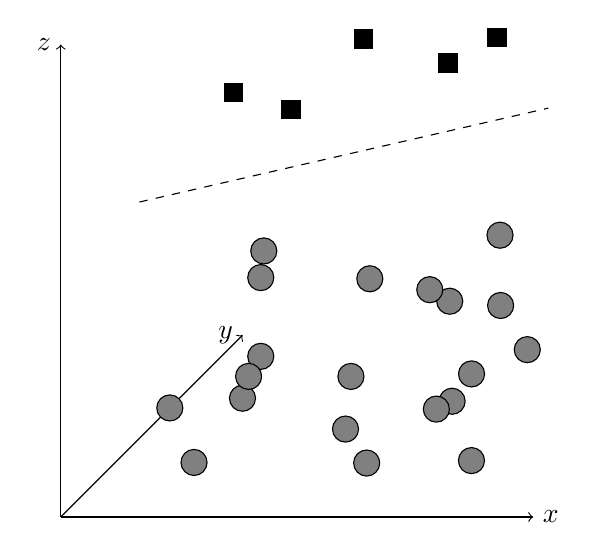
\begin{tikzpicture}
					\draw [->] (0,0,0) -- (6,0,0) node [at end, right] {$x$};
					\draw [->] (0,0,0) -- (0,6,0) node [at end, left] {$z$};
					\draw [->] (0,0,0) -- (0,0,-6) node [at end, left] {$y$};
					
					\node [black,circle,draw,fill=gray](s) at (1,1,-1){};
					\node [black,circle,draw,fill=gray](s) at (2,1.2,-0.8){};
					\node [black,circle,draw,fill=gray](s) at (1.5,0.5,-0.5){};
					\node [black,circle,draw,fill=gray](s) at (4,0.2,-5){};
					\node [black,circle,draw,fill=gray](s) at (2,1.1,-5){};
					\node [black,circle,draw,fill=gray](s) at (1,1.8,-4.1){};
					\node [black,circle,draw,fill=gray](s) at (3.5,0.3,-1){};
					\node [black,circle,draw,fill=gray](s) at (1,0.5,-4){};
					\node [black,circle,draw,fill=gray](s) at (4.6,0.1,-1.6){};
					\node [black,circle,draw,fill=gray](s) at (2.5,0,-2.9){};
					\node [black,circle,draw,fill=gray](s) at (1.5,0.9,-2.3){};
					\node [black,circle,draw,fill=gray](s) at (4.2,0.7,-2){};
					\node [black,circle,draw,fill=gray](s) at (4,0.6,-2){};
					\node [black,circle,draw,fill=gray](s) at (4,2,-4.1){};
					\node [black,circle,draw,fill=gray](s) at (3.3,1.4,-1){};
					\node [black,circle,draw,fill=gray](s) at (1,1.5,-4){};
					\node [black,circle,draw,fill=gray](s) at (3.4,1.2,-4){};
					\node [black,circle,draw,fill=gray](s) at (2.8,1,-4.9){};
					\node [black,circle,draw,fill=gray](s) at (3.6,0.2,-4.2){};
					\node [black,circle,draw,fill=gray](s) at (4.2,1.3,-3.6){};
					
					\node [draw,fill=black](s) at (2,4.25,-2.4){};
					\node [draw,fill=black](s) at (2.5,4.72,-3.5){};
					\node [draw,fill=black](s) at (3.8,4.65,-2.9){};
					\node [draw,fill=black](s) at (1.5,4.7,-1.8){};
					\node [draw,fill=black](s) at (4,4.55,-4){};
					
					\draw[dashed] (1,4,0) -- (6,5,-0.5);
				\end{tikzpicture}
			\end{minipage}
			\centering
			\caption{(a) Abbildung von möglichen, Objektlassen im zweidimensionalen Raum. Die Formen stellen jeweils Klassen dar, wie zum Beispiel die Klassen Hund und Person. (b) Darstellung der in a gezeigten Objektklassen im dreidimensionalen Raum. Die gestrichelte Linie deutet eine lineare Trennung an.}
			\label{fig: kerneltrick}
	\end{figure}
			
		Die \textit{HoG} Methode in Verbindung mit der beschriebenen \textit{SVM} ist ein weitverbreitetes Mittel zur Klassifikation \cite{hogsvmvscnn}. Die Publikation von \textit{Kibira} und \textit{Hasan} führt Vergleiche hinsichtlich der Trainingszeit und der Genauigkeit von \textit{HoG-SVM}-Kombinationen und Faltungsnetzwerken an \cite{hogsvmvscnn}. Letzteres weist im direkten Vergleich eine höhere Klassifikationsgenauigkeit bei verhältnismäßig längerer Trainingsdauer auf. Faltungsnetzwerke werden im folgenden Abschnitt behandelt. 
	
		\subsection{Objekterkennung durch neuronale Netze}
		\label{subsec: Objekterkennung durch neuronale Netze}
		Die bisher besten Ergebnisse in der Bildverarbeitung wurden durch die Abwandlung der neuronalen Netze, der sogenannten \textit{Convolutional Neural Networks} (CNN) erreicht \cite{deeplearning}. Derartige Netzwerke nutzen zur Verarbeitung der Eingangsdaten Faltungsoperationen statt der üblichen Matrizenmultiplikation \cite{deeplearning}. Diese werden auch als Konvolution bezeichnet. Der Aufbau eines CNNs setzt sich aus einer Merkmalsextraktion eines Bildes und die darauffolgende Klassifikation zusammen.\\ 
		
		\begin{figure}[H]
			\centering		
			\begin{tikzpicture}
				\pgfmathsetmacro{\cubex}{0.01}
				\pgfmathsetmacro{\cubey}{5}
				\pgfmathsetmacro{\cubez}{5}
				
				\begin{scope}[line width=0.2mm]
				\begin{scope}
				\clip[] (-0.8,0,0) -- ++(-\cubex,0,0) -- ++(0,-\cubey,0) -- ++(\cubex,0,0) -- cycle;
				\draw[fill=white] (-0.8,0,0) -- ++(-\cubex,0,0) -- ++(0,-\cubey,0) -- ++(\cubex,0,0) -- cycle;
				\end{scope}
				\begin{scope}
				\clip[] (-0.8,0,0) -- ++(0,0,-\cubez) -- ++(0,-\cubey,0) -- ++(0,0,\cubez) -- cycle;
				\draw[fill=white] (-0.8,0,0) -- ++(0,0,-\cubez) -- ++(0,-\cubey,0) -- ++(0,0,\cubez) -- cycle;
				\end{scope}
				\begin{scope}
				\clip[] (-0.8,0,0) -- ++(-\cubex,0,0) -- ++(0,0,-\cubez) -- ++(\cubex,0,0) -- cycle;
				\draw[fill=white] (-0.8,0,0) -- ++(-\cubex,0,0) -- ++(0,0,-\cubez) -- ++(\cubex,0,0) -- cycle;
				\end{scope}
				
				\begin{scope}
				\clip[] (-0.7,0,0) -- ++(-\cubex,0,0) -- ++(0,-\cubey,0) -- ++(\cubex,0,0) -- cycle;
				\draw[fill=white] (-0.7,0,0) -- ++(-\cubex,0,0) -- ++(0,-\cubey,0) -- ++(\cubex,0,0) -- cycle;
				\end{scope}
				\begin{scope}
				\clip[] (-0.7,0,0) -- ++(0,0,-\cubez) -- ++(0,-\cubey,0) -- ++(0,0,\cubez) -- cycle;
				\draw[fill=white] (-0.7,0,0) -- ++(0,0,-\cubez) -- ++(0,-\cubey,0) -- ++(0,0,\cubez) -- cycle;
				\end{scope}
				\begin{scope}
				\clip[] (-0.7,0,0) -- ++(-\cubex,0,0) -- ++(0,0,-\cubez) -- ++(\cubex,0,0) -- cycle;
				\draw[fill=white] (-0.7,0,0) -- ++(-\cubex,0,0) -- ++(0,0,-\cubez) -- ++(\cubex,0,0) -- cycle;
				\end{scope}
			
				\begin{scope}
					\clip[] (-0.6,0,0) -- ++(-\cubex,0,0) -- ++(0,-\cubey,0) -- ++(\cubex,0,0) -- cycle;
					\draw[fill=white] (-0.6,0,0) -- ++(-\cubex,0,0) -- ++(0,-\cubey,0) -- ++(\cubex,0,0) -- cycle;
				\end{scope}
				\begin{scope}
					\clip[] (-0.6,0,0) -- ++(0,0,-\cubez) -- ++(0,-\cubey,0) -- ++(0,0,\cubez) -- cycle;
					\draw[fill=white] (-0.6,0,0) -- ++(0,0,-\cubez) -- ++(0,-\cubey,0) -- ++(0,0,\cubez) -- cycle;
				\end{scope}
				\begin{scope}
					\clip[] (-0.6,0,0) -- ++(-\cubex,0,0) -- ++(0,0,-\cubez) -- ++(\cubex,0,0) -- cycle;
					\draw[fill=white] (-0.6,0,0) -- ++(-\cubex,0,0) -- ++(0,0,-\cubez) -- ++(\cubex,0,0) -- cycle;
				\end{scope}	
				
				\begin{scope}
					\node[rotate=-22] (png) at (0.35,-1.8) {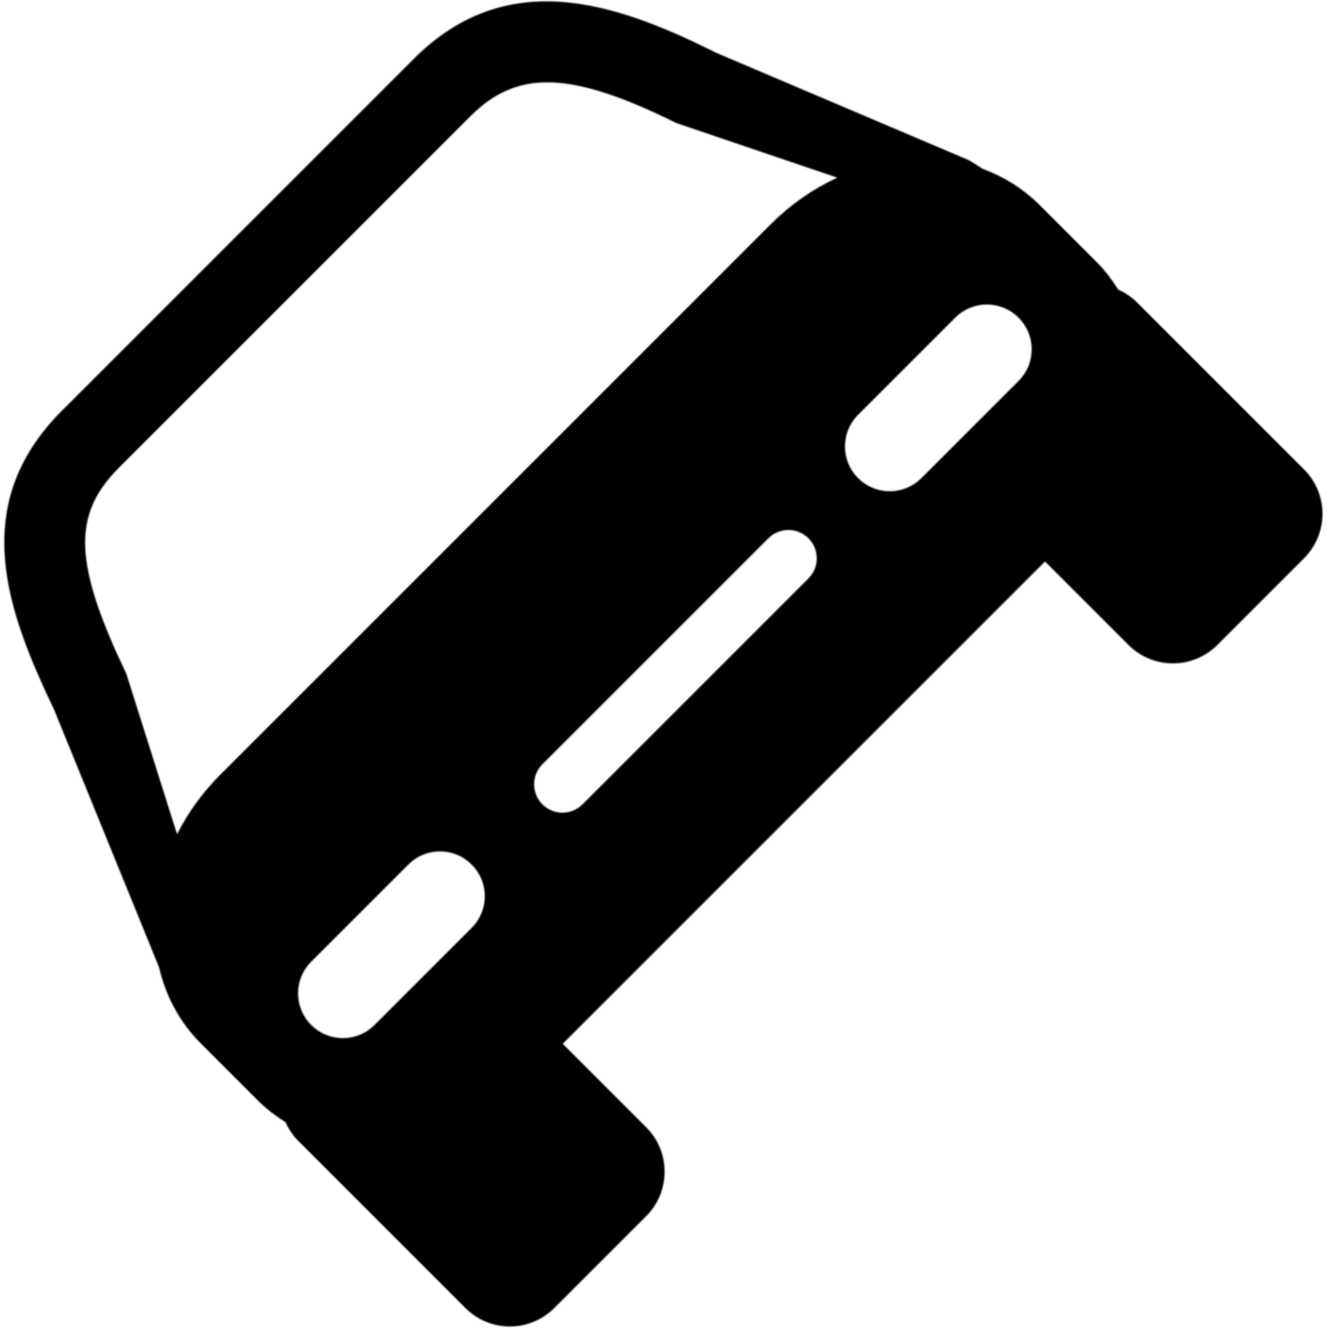
\includegraphics[height=3cm, width=1.5cm]{Bilder/png.png}};
				\end{scope}
				
				\pgfmathsetmacro{\cubey}{1}
				\pgfmathsetmacro{\cubez}{1}
				\pgfmathsetmacro{\x}{0.3}
				\pgfmathsetmacro{\y}{-2.3}
				
				\begin{scope}
					\clip[] (\x,\y,0) -- ++(0,0,-\cubez) -- ++(0,-\cubey,0) -- ++(0,0,\cubez) -- cycle;
					\draw[fill=white] (\x,\y,0) -- ++(0,0,-\cubez) -- ++(0,-\cubey,0) -- ++(0,0,\cubez) -- cycle;
				\end{scope}
				
				\draw[] (\x,\y-0.014,0) -- (1.809,-2.299,0);
				\draw[] (\x-0.002,\y-0.014,-\cubez) -- (1.801,-2.312,-0.5);
				\draw[] (\x-0.003,\y+0.005-\cubey,-\cubez) -- (1.799,-2.289-0.5,-0.5);
				\draw[] (\x+0.002,\y+0.009-\cubey,0) -- (1.805,-2.286-0.5,0);
				
				\pgfmathsetmacro{\cubey}{0.5}
				\pgfmathsetmacro{\cubez}{0.5}
				\pgfmathsetmacro{\x}{1.8}
				\pgfmathsetmacro{\y}{-2.3}
				
				\begin{scope}
					\clip[] (\x,\y,0) -- ++(0,0,-\cubez) -- ++(0,-\cubey,0) -- ++(0,0,\cubez) -- cycle;
					\draw[] (\x,\y,0) -- ++(0,0,-\cubez) -- ++(0,-\cubey,0) -- ++(0,0,\cubez) -- cycle;
				\end{scope}
				
				
				
				\pgfmathsetmacro{\cubex}{2}
				\pgfmathsetmacro{\cubey}{3}
				\pgfmathsetmacro{\cubez}{3}
				\pgfmathsetmacro{\x}{3.6}
				\pgfmathsetmacro{\y}{-0.5}
				
				\begin{scope}
					\clip[] (\x,\y,0) -- ++(-\cubex,0,0) -- ++(0,-\cubey,0) -- ++(\cubex,0,0) -- cycle;
					\draw[] (\x,\y,0) -- ++(-\cubex,0,0) -- ++(0,-\cubey,0) -- ++(\cubex,0,0) -- cycle;
				\end{scope}
				\begin{scope}
					\clip[] (\x,\y,0) -- ++(0,0,-\cubez) -- ++(0,-\cubey,0) -- ++(0,0,\cubez) -- cycle;
					\draw[] (\x,\y,0) -- ++(0,0,-\cubez) -- ++(0,-\cubey,0) -- ++(0,0,\cubez) -- cycle;
				\end{scope}
				\begin{scope}
					\clip[] (\x,\y,0) -- ++(-\cubex,0,0) -- ++(0,0,-\cubez) -- ++(\cubex,0,0) -- cycle;
					\draw[] (\x,\y,0) -- ++(-\cubex,0,0) -- ++(0,0,-\cubez) -- ++(\cubex,0,0) -- cycle;
				\end{scope}	
				\begin{scope}
					\clip[] (\x,\y,0-\cubez) -- ++(-\cubex,0,0) -- ++(0,-\cubey,0) -- ++(\cubex,0,0) -- cycle;
					\draw[] (\x,\y,0-\cubez) -- ++(-\cubex,0,0) -- ++(0,-\cubey,0) -- ++(\cubex,0,0) -- cycle;
				\end{scope}	
				\begin{scope}
					\clip[] (\x,\y-\cubey,0) -- ++(-\cubex,0,0) -- ++(0,0,-\cubez) -- ++(\cubex,0,0) -- cycle;
					\draw[] (\x,\y-\cubey,0) -- ++(-\cubex,0,0) -- ++(0,0,-\cubez) -- ++(\cubex,0,0) -- cycle;
				\end{scope}	
			
				\pgfmathsetmacro{\cubey}{1}
				\pgfmathsetmacro{\cubez}{1}
				\pgfmathsetmacro{\x}{3.8}
				\pgfmathsetmacro{\y}{-2}
				
				\begin{scope}
					\clip[] (\x,\y,0) -- ++(0,0,-\cubez) -- ++(0,-\cubey,0) -- ++(0,0,\cubez) -- cycle;
					\draw[] (\x,\y,0) -- ++(0,0,-\cubez) -- ++(0,-\cubey,0) -- ++(0,0,\cubez) -- cycle;
					
				\end{scope}
					\draw[] (\x-0.003,\y-0.01,0) -- (7.16,-2.01,0);
					\draw[] (\x,\y-0.02,-\cubez) -- (7.165,-1.999,-0.2);
					\draw[] (\x-0.005,\y-0.00-\cubey,-\cubez) -- (7.165,-2.02-0.2,-0.2);
					\draw[] (\x-0.001,\y+0.001-\cubey,0) -- (7.165,-2.02-0.2,0);
					
					
				\pgfmathsetmacro{\cubex}{2}
				\pgfmathsetmacro{\cubey}{2}
				\pgfmathsetmacro{\cubez}{2}
				\pgfmathsetmacro{\x}{7}
				\pgfmathsetmacro{\y}{-1}
				
				\begin{scope}
					\clip[] (\x,\y,0) -- ++(-\cubex,0,0) -- ++(0,-\cubey,0) -- ++(\cubex,0,0) -- cycle;
					\draw[] (\x,\y,0) -- ++(-\cubex,0,0) -- ++(0,-\cubey,0) -- ++(\cubex,0,0) -- cycle;
				\end{scope}
				\begin{scope}
					\clip[] (\x,\y,0) -- ++(0,0,-\cubez) -- ++(0,-\cubey,0) -- ++(0,0,\cubez) -- cycle;
					\draw[] (\x,\y,0) -- ++(0,0,-\cubez) -- ++(0,-\cubey,0) -- ++(0,0,\cubez) -- cycle;
				\end{scope}
				\begin{scope}
					\clip[] (\x,\y,0) -- ++(-\cubex,0,0) -- ++(0,0,-\cubez) -- ++(\cubex,0,0) -- cycle;
					\draw[] (\x,\y,0) -- ++(-\cubex,0,0) -- ++(0,0,-\cubez) -- ++(\cubex,0,0) -- cycle;
				\end{scope}	
				\begin{scope}
					\clip[] (\x,\y,0-\cubez) -- ++(-\cubex,0,0) -- ++(0,-\cubey,0) -- ++(\cubex,0,0) -- cycle;
					\draw[] (\x,\y,0-\cubez) -- ++(-\cubex,0,0) -- ++(0,-\cubey,0) -- ++(\cubex,0,0) -- cycle;
				\end{scope}	
				\begin{scope}
					\clip[] (\x,\y-\cubey,0) -- ++(-\cubex,0,0) -- ++(0,0,-\cubez) -- ++(\cubex,0,0) -- cycle;
					\draw[] (\x,\y-\cubey,0) -- ++(-\cubex,0,0) -- ++(0,0,-\cubez) -- ++(\cubex,0,0) -- cycle;
				\end{scope}
				
				\pgfmathsetmacro{\cubey}{0.25}
				\pgfmathsetmacro{\cubez}{0.25}
				\pgfmathsetmacro{\x}{7.15}
				\pgfmathsetmacro{\y}{-2}
				
				\begin{scope}
					\clip[] (\x,\y,0) -- ++(0,0,-\cubez) -- ++(0,-\cubey,0) -- ++(0,0,\cubez) -- cycle;
					\draw[] (\x,\y,0) -- ++(0,0,-\cubez) -- ++(0,-\cubey,0) -- ++(0,0,\cubez) -- cycle;
				\end{scope}
			
				\pgfmathsetmacro{\cubex}{2}
				\pgfmathsetmacro{\cubey}{0.8}
				\pgfmathsetmacro{\cubez}{0.8}
				\pgfmathsetmacro{\x}{7.35}
				\pgfmathsetmacro{\y}{-0.9}
				
				\begin{scope}
					\clip[] (\x,\y,0) -- ++(-\cubex,0,0) -- ++(0,-\cubey,0) -- ++(\cubex,0,0) -- cycle;
					\draw[] (\x,\y,0) -- ++(-\cubex,0,0) -- ++(0,-\cubey,0) -- ++(\cubex,0,0) -- cycle;
				\end{scope}
				\begin{scope}
					\clip[] (\x,\y,0) -- ++(0,0,-\cubez) -- ++(0,-\cubey,0) -- ++(0,0,\cubez) -- cycle;
					\draw[] (\x,\y,0) -- ++(0,0,-\cubez) -- ++(0,-\cubey,0) -- ++(0,0,\cubez) -- cycle;
				\end{scope}
				\begin{scope}
					\clip[] (\x,\y,0) -- ++(-\cubex,0,0) -- ++(0,0,-\cubez) -- ++(\cubex,0,0) -- cycle;
					\draw[] (\x,\y,0) -- ++(-\cubex,0,0) -- ++(0,0,-\cubez) -- ++(\cubex,0,0) -- cycle;
				\end{scope}	
				\begin{scope}
					\clip[] (\x,\y,0-\cubez) -- ++(-\cubex,0,0) -- ++(0,-\cubey,0) -- ++(\cubex,0,0) -- cycle;
					\draw[] (\x,\y,0-\cubez) -- ++(-\cubex,0,0) -- ++(0,-\cubey,0) -- ++(\cubex,0,0) -- cycle;
				\end{scope}	
				\begin{scope}
					\clip[] (\x,\y-\cubey,0) -- ++(-\cubex,0,0) -- ++(0,0,-\cubez) -- ++(\cubex,0,0) -- cycle;
					\draw[] (\x,\y-\cubey,0) -- ++(-\cubex,0,0) -- ++(0,0,-\cubez) -- ++(\cubex,0,0) -- cycle;
				\end{scope}
			
				\draw[] (\x-0.003,\y-0.015,0) -- (8.515,-1.09,0);
				\draw[] (\x-0.01,\y-0.01,-\cubez) -- (8.5,-1.115,-0.2);
				\draw[] (\x,\y-\cubey,-\cubez) -- (8.499,-1.09-0.2,-0.2);
				\draw[] (\x,\y-\cubey,0) -- (8.505,-1.085-0.2,0);
			
				\pgfmathsetmacro{\cubey}{0.2}
				\pgfmathsetmacro{\cubez}{0.2}
				\pgfmathsetmacro{\x}{8.5}
				\pgfmathsetmacro{\y}{-1.1}
				
				\begin{scope}
					\clip[] (\x,\y,0) -- ++(0,0,-\cubez) -- ++(0,-\cubey,0) -- ++(0,0,\cubez) -- cycle;
					\draw[] (\x,\y,0) -- ++(0,0,-\cubez) -- ++(0,-\cubey,0) -- ++(0,0,\cubez) -- cycle;
				\end{scope}
				
				
			
				\pgfmathsetmacro{\cubex}{0.5}
				\pgfmathsetmacro{\cubey}{0.5}
				\pgfmathsetmacro{\cubez}{0.5}
				
				
				\begin{scope}
					\clip[] (11.5,1,0) -- ++(-\cubex,0,0) -- ++(0,-\cubey,0) -- ++(\cubex,0,0) -- cycle;
					\draw[fill=white] (11.5,1,0) -- ++(-\cubex,0,0) -- ++(0,-\cubey,0) -- ++(\cubex,0,0) -- cycle;
				\end{scope}
				\begin{scope}
					\clip[] (11.5,0.5,0) -- ++(-\cubex,0,0) -- ++(0,-\cubey,0) -- ++(\cubex,0,0) -- cycle;
					\draw[fill=white] (11.5,0.5,0) -- ++(-\cubex,0,0) -- ++(0,-\cubey,0) -- ++(\cubex,0,0) -- cycle;
				\end{scope}
				\begin{scope}
					\clip[] (11.5,0,0) -- ++(-\cubex,0,0) -- ++(0,-\cubey,0) -- ++(\cubex,0,0) -- cycle;
					\draw[fill=white] (11.5,0,0) -- ++(-\cubex,0,0) -- ++(0,-\cubey,0) -- ++(\cubex,0,0) -- cycle;
				\end{scope}
				\begin{scope}
					\clip[] (11.5,-0.5,0) -- ++(-\cubex,0,0) -- ++(0,-\cubey,0) -- ++(\cubex,0,0) -- cycle;
					\draw[fill=white] (11.5,-0.5,0) -- ++(-\cubex,0,0) -- ++(0,-\cubey,0) -- ++(\cubex,0,0) -- cycle;
				\end{scope}
				\begin{scope}
					\clip[] (11.5,-1,0) -- ++(-\cubex,0,0) -- ++(0,-\cubey,0) -- ++(\cubex,0,0) -- cycle;
					\draw[fill=white] (11.5,-1,0) -- ++(-\cubex,0,0) -- ++(0,-\cubey,0) -- ++(\cubex,0,0) -- cycle;
				\end{scope}
				\begin{scope}
					\clip[] (11.5,-1.5,0) -- ++(-\cubex,0,0) -- ++(0,-\cubey,0) -- ++(\cubex,0,0) -- cycle;
					\draw[fill=white] (11.5,-1.5,0) -- ++(-\cubex,0,0) -- ++(0,-\cubey,0) -- ++(\cubex,0,0) -- cycle;
				\end{scope}
				\begin{scope}
					\clip[] (11.5,-2,0) -- ++(-\cubex,0,0) -- ++(0,-\cubey,0) -- ++(\cubex,0,0) -- cycle;
					\draw[fill=white] (11.5,-2,0) -- ++(-\cubex,0,0) -- ++(0,-\cubey,0) -- ++(\cubex,0,0) -- cycle;
				\end{scope}
				\begin{scope}
					\clip[] (11.5,-2.5,0) -- ++(-\cubex,0,0) -- ++(0,-\cubey,0) -- ++(\cubex,0,0) -- cycle;
					\draw[fill=white] (11.5,-2.5,0) -- ++(-\cubex,0,0) -- ++(0,-\cubey,0) -- ++(\cubex,0,0) -- cycle;
				\end{scope}
				\begin{scope}
					\clip[] (11.5,-4,0) -- ++(-\cubex,0,0) -- ++(0,-\cubey,0) -- ++(\cubex,0,0) -- cycle;
					\draw[fill=white] (11.5,-4,0) -- ++(-\cubex,0,0) -- ++(0,-\cubey,0) -- ++(\cubex,0,0) -- cycle;
				\end{scope}
			
				
					\begin{scope}
					\clip[] (10,1,0) -- ++(-\cubex,0,0) -- ++(0,-\cubey,0) -- ++(\cubex,0,0) -- cycle;
					\draw[fill=white] (10,1,0) -- ++(-\cubex,0,0) -- ++(0,-\cubey,0) -- ++(\cubex,0,0) -- cycle;
				\end{scope}
				\begin{scope}
					\clip[] (10,0.5,0) -- ++(-\cubex,0,0) -- ++(0,-\cubey,0) -- ++(\cubex,0,0) -- cycle;
					\draw[fill=white] (10,0.5,0) -- ++(-\cubex,0,0) -- ++(0,-\cubey,0) -- ++(\cubex,0,0) -- cycle;
				\end{scope}
				\begin{scope}
					\clip[] (10,0,0) -- ++(-\cubex,0,0) -- ++(0,-\cubey,0) -- ++(\cubex,0,0) -- cycle;
					\draw[fill=white] (10,0,0) -- ++(-\cubex,0,0) -- ++(0,-\cubey,0) -- ++(\cubex,0,0) -- cycle;
				\end{scope}
				\begin{scope}
					\clip[] (10,-0.5,0) -- ++(-\cubex,0,0) -- ++(0,-\cubey,0) -- ++(\cubex,0,0) -- cycle;
					\draw[fill=white] (10,-0.5,0) -- ++(-\cubex,0,0) -- ++(0,-\cubey,0) -- ++(\cubex,0,0) -- cycle;
				\end{scope}
				\begin{scope}
					\clip[] (10,-1,0) -- ++(-\cubex,0,0) -- ++(0,-\cubey,0) -- ++(\cubex,0,0) -- cycle;
					\draw[fill=white] (10,-1,0) -- ++(-\cubex,0,0) -- ++(0,-\cubey,0) -- ++(\cubex,0,0) -- cycle;
				\end{scope}
				\begin{scope}
					\clip[] (10,-1.5,0) -- ++(-\cubex,0,0) -- ++(0,-\cubey,0) -- ++(\cubex,0,0) -- cycle;
					\draw[fill=white] (10,-1.5,0) -- ++(-\cubex,0,0) -- ++(0,-\cubey,0) -- ++(\cubex,0,0) -- cycle;
				\end{scope}
				\begin{scope}
					\clip[] (10,-2,0) -- ++(-\cubex,0,0) -- ++(0,-\cubey,0) -- ++(\cubex,0,0) -- cycle;
					\draw[fill=white] (10,-2,0) -- ++(-\cubex,0,0) -- ++(0,-\cubey,0) -- ++(\cubex,0,0) -- cycle;
				\end{scope}
				\begin{scope}
					\clip[] (10,-2.5,0) -- ++(-\cubex,0,0) -- ++(0,-\cubey,0) -- ++(\cubex,0,0) -- cycle;
					\draw[fill=white] (10,-2.5,0) -- ++(-\cubex,0,0) -- ++(0,-\cubey,0) -- ++(\cubex,0,0) -- cycle;
				\end{scope}
				\begin{scope}
					\clip[] (10,-4,0) -- ++(-\cubex,0,0) -- ++(0,-\cubey,0) -- ++(\cubex,0,0) -- cycle;
					\draw[fill=white] (10,-4,0) -- ++(-\cubex,0,0) -- ++(0,-\cubey,0) -- ++(\cubex,0,0) -- cycle;
				\end{scope}
			
			
					\begin{scope}
					\clip[] (13,1,0) -- ++(-\cubex,0,0) -- ++(0,-\cubey,0) -- ++(\cubex,0,0) -- cycle;
					\draw[fill=white] (13,1,0) -- ++(-\cubex,0,0) -- ++(0,-\cubey,0) -- ++(\cubex,0,0) -- cycle;
				\end{scope}
				\begin{scope}
					\clip[] (13,0.5,0) -- ++(-\cubex,0,0) -- ++(0,-\cubey,0) -- ++(\cubex,0,0) -- cycle;
					\draw[fill=white] (13,0.5,0) -- ++(-\cubex,0,0) -- ++(0,-\cubey,0) -- ++(\cubex,0,0) -- cycle;
				\end{scope}
				\begin{scope}
					\clip[] (13,0,0) -- ++(-\cubex,0,0) -- ++(0,-\cubey,0) -- ++(\cubex,0,0) -- cycle;
					\draw[fill=white] (13,0,0) -- ++(-\cubex,0,0) -- ++(0,-\cubey,0) -- ++(\cubex,0,0) -- cycle;
				\end{scope}
				\begin{scope}
					\clip[] (13,-0.5,0) -- ++(-\cubex,0,0) -- ++(0,-\cubey,0) -- ++(\cubex,0,0) -- cycle;
					\draw[fill=white] (13,-0.5,0) -- ++(-\cubex,0,0) -- ++(0,-\cubey,0) -- ++(\cubex,0,0) -- cycle;
				\end{scope}
				\begin{scope}
					\clip[] (13,-1,0) -- ++(-\cubex,0,0) -- ++(0,-\cubey,0) -- ++(\cubex,0,0) -- cycle;
					\draw[fill=white] (13,-1,0) -- ++(-\cubex,0,0) -- ++(0,-\cubey,0) -- ++(\cubex,0,0) -- cycle;
				\end{scope}
				\begin{scope}
					\clip[] (13,-1.5,0) -- ++(-\cubex,0,0) -- ++(0,-\cubey,0) -- ++(\cubex,0,0) -- cycle;
					\draw[fill=white] (13,-1.5,0) -- ++(-\cubex,0,0) -- ++(0,-\cubey,0) -- ++(\cubex,0,0) -- cycle;
				\end{scope}
				\begin{scope}
					\clip[] (13,-2,0) -- ++(-\cubex,0,0) -- ++(0,-\cubey,0) -- ++(\cubex,0,0) -- cycle;
					\draw[fill=white] (13,-2,0) -- ++(-\cubex,0,0) -- ++(0,-\cubey,0) -- ++(\cubex,0,0) -- cycle;
				\end{scope}
				\begin{scope}
					\clip[] (13,-2.5,0) -- ++(-\cubex,0,0) -- ++(0,-\cubey,0) -- ++(\cubex,0,0) -- cycle;
					\draw[fill=white] (13,-2.5,0) -- ++(-\cubex,0,0) -- ++(0,-\cubey,0) -- ++(\cubex,0,0) -- cycle;
				\end{scope}
				\begin{scope}
					\clip[] (13,-4,0) -- ++(-\cubex,0,0) -- ++(0,-\cubey,0) -- ++(\cubex,0,0) -- cycle;
					\draw[fill=white] (13,-4,0) -- ++(-\cubex,0,0) -- ++(0,-\cubey,0) -- ++(\cubex,0,0) -- cycle;
				\end{scope}
				
				\begin{scope}
				\node[rotate=90] (S1) at (9.75,-3.5) {$\cdots$};
				\node[rotate=90] (S1) at (11.25,-3.5) {$\cdots$};
				\node[rotate=90] (S1) at (12.75,-3.5) {$\cdots$};
				\node[rotate=90] (S1) at (13.6,-1.22) {$\cdots$};
				\node[] (S1) at (8.6,-2) {$\cdots$};
%				\node[rotate=90] (S2) at (5.3,-2.59) {$\cdots$};
%				\draw[gray,thick,->,>=stealth](-0.5,0.4) -- (-0.5,2.3) -- (1.6,2.3);
%				\draw[gray,thick,->,>=stealth](-0.7,-1) -- (1.6,-1);
%				\draw[gray,thick,->,>=stealth](-0.1,-1.1) -- (-0.1,-4.7) -- (1.6,-4.7);
%				\draw[gray,thick,->,>=stealth](6,2.3) -- (8.3,2.3) -- (8.3,0.4);
%				\draw[gray,thick,->,>=stealth](6,-1) -- (8.1,-1);
%				\draw[gray,thick,->,>=stealth](6,-4.7) -- (8.7,-4.7) -- (8.7,-1);
%				\draw[gray,thick,<->,>=stealth](2.6,2.3) -- (4.6,2.3);
%				\draw[gray,thick,<->,>=stealth](2.6,-1) -- (4.6,-1);
%				\draw[gray,thick,<->,>=stealth](2.6,-4.7) -- (4.6,-4.7);
%				\draw[gray,thick,<->,>=stealth](9.8,-0.5) -- (11.3,-0.5);
				\node[anchor=west] (m) at (13,0.72) {Auto};
				\node[anchor=west] (m) at (13,0.22) {Person};
				\node[anchor=west] (m) at (13,-0.28) {Baum};
				
				\draw (9.75,0.75) -- (8.5,0);
				\draw (9.75,-4.25) -- (8.5,-3.5);
				
				\draw (10.1,0.75) -- (10.9,0.75);
				\draw (10.1,0.75) -- (10.9,-0.75);
				\draw (10.1,0.75) -- (10.9,-4.25);
				\draw (10.1,-4.25) -- (10.9,0.75);
				\draw (10.1,-4.25) -- (10.9,-2.75);
				\draw (10.1,-4.25) -- (10.9,-4.25);
				
				\draw (11.6,0.75) -- (12.4,0.75);
				\draw (11.6,0.25) -- (12.4,0.25);
				\draw (11.6,-0.25) -- (12.4,-0.25);
				
				
				\node[anchor=north west] (m) at (0,-5) {Bild};
				\node[anchor=north west] (m) at (2.5,-5) {Faltung};
				\node[anchor=north west] (m) at (5.5,-5) {Pooling};
		
				\node[anchor=north west] (m) at (12,-5) {Softmax};
				\node[anchor=north west] (m) at (9.4,-5) {\makecell{vollständig\\verbundene\\Schicht}};
				
				\draw[thick,decorate,decoration={brace,amplitude=12pt}] ($(9,-7)$) -- ($(-1,-7)$) node[midway, below,yshift=-12pt,]{Merkmalsextraktion};
				\draw[thick,decorate,decoration={brace,amplitude=12pt}] ($(13.5,-7)$) -- ($(9.5,-7)$) node[midway, below,yshift=-12pt,]{Klassifikation};
%				\node[] (m) at (12.7,1) {$N$};
%				\node[] (m) at (1.1,-0.3) {$D_F$};
%				\node[] (m) at (0.7,-1.8) {$D_F$};
%				\node[] (m) at (3.7,-1.8) {\Umbruch{$D_K\times D_K$ Faltung} };
%				\node[] (m) at (10.55,0.3) {\Umbruch{$1\times 1$ Faltung} };
				\end{scope}
				\end{scope}
				
				
			\end{tikzpicture}
			\caption{Prinzipdarstellung eines Faltungsnetzwerks. Fortsetzungen werden mit drei aufeinander folgenden Punkten gekennzeichnet. Durch rechteckige Formen werden Schichten dargestellt. Angedeutet durch Pyramidenformen werden Prozesse der Faltung und des Poolings dargestellt. Darstellung adaptiert aus \cite{carpng,todasc}.}
			\label{fig: depthwise conv }
		\end{figure}
		
	 	
	
		Eine Einheit der Merkmalsextraktion besteht im grundlegenden Fall aus drei Unterschichten. Dabei können sich diese innerhalb der Merkmalsextraktion hintereinander wiederholen. Dies hat jedoch Einfluss auf die Eigenschaften eines Netzes. Die erste Unterschicht führt Faltungsprozesse mit den Eingangsdaten durch \cite{deeplearning}. Im zweiten Schritt wird eine nichtlineare Aktivierungsfunktion wie zum Beispiel der \textit{Rectified Linear Unit} (ReLU) Funktion auf die Ausgangsdaten der Konvolutionsschicht angewendet. In der dritten Unterschicht wird das sogenannte \textit{Pooling} durchgeführt. In einigen Fällen wird die Zusammensetzung der drei Stufen als Konvolutionsschicht bezeichnet, obwohl lediglich die erste Unterschicht die Konvolution vollzieht \cite{deeplearning}. Im Laufe dieses Abschnitts wird auf die Motivation der Nutzung und der Funktionsweise eines CNNs eingegangen.\\
		
		Es gibt drei Grundsätze für die Nutzung von Faltung in einem neuronalen Netz. Hierzu gehören die eingeschränkte Konnektivität, die Parameterverteilung und die äquivariante Darstellung \cite{deeplearning}. Im folgenden Abschnitt werden diese Punkte näher erläutert.\\
		
			\tikzset{%
			every neuron/.style={
				rectangle,
				draw,
				minimum size=1cm
			},
			neuron missing/.style={
				draw=none, 
				%scale=4,
				%rotate=90,
				%yshift=1,
				%text height=0.333cm,
				%execute at begin node=\color{black}$\cdots$
			},
		}
		\begin{figure}[H]
			\centering
			
			
			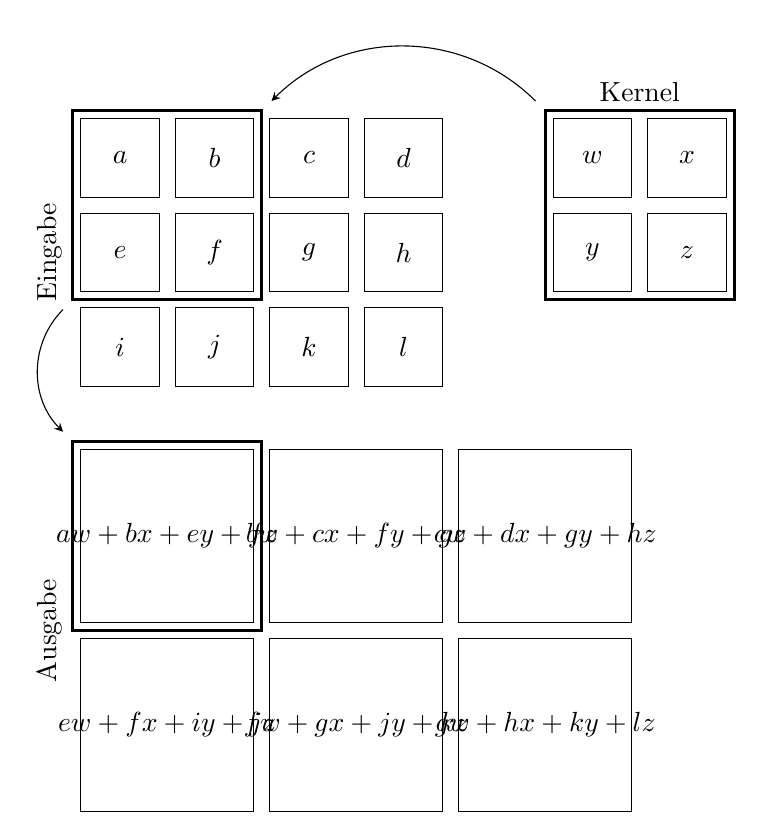
\begin{tikzpicture}[x=1.5cm, y=1.2cm, >=stealth]
			
			\foreach \m/\l [count=\y] in {1,2,3}
			\node [every neuron/.try, neuron \m/.try] (input-\m) at (0,2.5-\y) {};
			
			\foreach \m [count=\y] in {1,2,3}
			\node [every neuron/.try, neuron \m/.try ] (hidden1-\m) at (0.8,2.5-\y) {};
			
			\foreach \m [count=\y] in {1,2,3}
			\node [every neuron/.try, neuron \m/.try ] (hidden2-\m) at (1.6,2.5-\y) {};
			
			\foreach \m [count=\y] in {1,2,3}
			\node [every neuron/.try, neuron \m/.try ] (output-\m) at (2.4,2.5-\y) {};
			
			\foreach \m [count=\y] in {1,2}
			\node [every neuron/.try, neuron \m/.try ] (output-\m) at (4,2.5-\y) {};
			
			\foreach \m [count=\y] in {1,2}
			\node [every neuron/.try, neuron \m/.try ] (output-\m) at (4.8,2.5-\y) {};
			
			
			
			
			
			\foreach \m/\l [count=\y] in {0,1.6,3.2}
			\node[draw,rectangle,minimum width=2.2cm,minimum height=2.2cm] at (0.4+\m,-2.5) {};
			\foreach \m/\l [count=\y] in {0,1.6,3.2}
			\node[draw,rectangle,minimum width=2.2cm,minimum height=2.2cm] at (0.4+\m,-4.5) {};
			
			\node[] at (0.4,-2.5) {\Umbruch{$aw + bx + ey + fz$}};
			\node[] at (2,-2.5) {\Umbruch{$bw + cx + fy + gz$}};
			\node[] at (3.6,-2.5) {\Umbruch{$cw + dx + gy + hz$}};
			\node[] at (0.4,-4.5) {\Umbruch{$ew + fx + iy + jz$}};
			\node[] at (2,-4.5) {\Umbruch{$fw + gx + jy + kz$}};
			\node[] at (3.6,-4.5) {\Umbruch{$gw + hx + ky + lz$}};
			
			
			\node[] at (0,1.5) {$a$};
			\node[] at (0.8,1.5) {$b$};
			\node[] at (1.6,1.5) {$c$};
			\node[] at (2.4,1.5) {$d$};
			\node[] at (0,0.5) {$e$};
			\node[] at (0.8,0.5) {$f$};
			\node[] at (1.6,0.5) {$g$};
			\node[] at (2.4,0.5) {$h$};
			\node[] at (0,-0.5) {$i$};
			\node[] at (0.8,-0.5) {$j$};
			\node[] at (1.6,-0.5) {$k$};
			\node[] at (2.4,-0.5) {$l$};
			\node[] at (4,1.5) {$w$};
			\node[] at (4.8,1.5) {$x$};
			\node[] at (4,0.5) {$y$};
			\node[] at (4.8,0.5) {$z$};
			
			\node[rotate=90] at (-0.6,0.5) {Eingabe};
			\node[rotate=90] at (-0.6,-3.5) {Ausgabe};
			\node[] at (4.4,2.2) {Kernel};
			
			\node[] (S1) at (3.6,2){};
			\node[] (S2) at (1.2,2){};
			\node[] (S3) at (-0.4,-0.0){};
			\node[] (S4) at (-0.4,-1.5){};
			\node[very thick,draw,rectangle,minimum width=2.4cm,minimum height=2.4cm] at (0.4,-2.5) {};
			\node[very thick,draw,rectangle,minimum width=2.4cm,minimum height=2.4cm] at (4.4,1) {};
			\node[very thick,draw,rectangle,minimum width=2.4cm,minimum height=2.4cm] at (0.4,1) {};
			\draw [->, bend angle=45, bend right]  (S1) to (S2);
			\draw [->, bend angle=45, bend right]  (S3) to (S4);
		
			
			
			
			
		
			\end{tikzpicture}
			\caption{Prinzipielle Darstellung des Faltungsprozesses. Mit einem Quadrat umrandete Buchstaben stellen Daten wie zum Beispiel ein Pixel dar. Der Kernel fasst in dieser Abbildung beispielsweise vier Daten zu einer Information zusammen und gibt diese aus. Adaptiert aus \cite{deeplearning}.}
			\label{fig: faltung }
		\end{figure}
		
		
		Während der Konvolution werden eingehende Daten in Filter, sogenannte Kernels, eingegeben. Abbildung \ref{fig: faltung } zeigt den prinzipiellen Vorgang der Faltung. Hierbei wird die Matrix des Kernels mit der Eingabematrix elementweise multipliziert und erzeugt die gezeigte Ausgabe. Die Konfiguration des Kernels ist beispielhaft mit $w$, $x$, $y$ und $z$ dargestellt. Eingehende Datenpunkte sind hier mit den Buchstaben $a$ bis $l$ gekennzeichnet. Die Filter extrahieren bestimmte Merkmale je nach Konfiguration, wie im unteren Teil der Abbildung als Ausgabe dargestellt. So können verschiedene Schichten diverse Merkmale extrahieren. Die Ausgänge der Schichten üblicher, neuronaler Netze sind mit jedem Eingang der folgenden Schicht verknüpft. Ein typischer Aufbau wurde bereits in Abschnitt \ref{subsec: Eigenschaften von neuronalen Netzen} in Abbildung \ref{fig: neuronales netz } gezeigt. Wird bei derartigen Netzen eine Schicht mit $n$ Ausgaben und eine mit $m$ Eingaben verknüpft, werden $m \cdot n$ Parameter benötigt \cite{deeplearning}. Durch den Faltungsprozess wird diese Konnektivität eingeschränkt. Beispielsweise wird der Datenpunkt $b$ der Eingabe aus der Darstellung \ref{fig: faltung } lediglich in zwei von sechs Datenpunkten der Ausgabe berücksichtigt. Die Ausmaße der eingeschränkten Konnektivität lassen sich in der folgenden Abbildung \ref{fig: eingeschränkte konnektivität} verdeutlichen. Die Eingabepunkte $I_n$ geben je nach Netzart ihre Informationen an alle oder benachbarten Ausgabepunkte $O_n$ weiter. Die Einschränkung der Konnektivität hängt von der Dimension des Kernels ab. Folglich nehmen CNNs deutlich weniger Speicher ein im Vergleich zu herkömmlichen KNNs \cite{deeplearning}. Gleichzeitig wird durch die Faltung eine höhere statistische Effizienz erreicht \cite{deeplearning}.\\
		
	
			\tikzset{%
			every neuron/.style={
				circle,
				draw,
				minimum size=1cm
			},
			neuron missing/.style={
				draw=none, 
				%scale=4,
				%rotate=90,
				%yshift=1,
				%text height=0.333cm,
				%execute at begin node=\color{black}$\cdots$
			},
		}
	
		
		\begin{figure}[H]
			\centering
			
			
			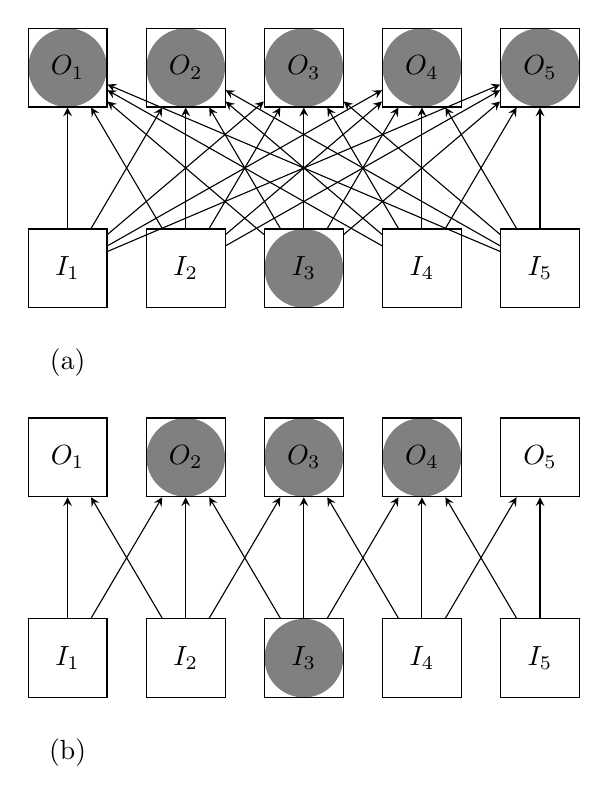
\begin{tikzpicture}[x=1.5cm, y=1.5cm, >=stealth]
			
			\foreach \m/\l [count=\y] in {1,2,3,4,5}
			\draw[gray,fill=gray](0+\y,2.5)circle(14pt);
			
			\foreach \m/\l [count=\y] in {2,3,4}
			\draw[gray,fill=gray](0+\m,-0.8)circle(14pt);
			
			\draw[gray,fill=gray](3,0.8)circle(14pt);
			\draw[gray,fill=gray](3,-2.5)circle(14pt);
			
			\foreach \m/\l [count=\y] in {1,2,3,4,5}
			\node [every neuron/.try, neuron \m/.try] (eins-\m) at (0+\y,2.5) {$O_\y$};
			
			\foreach \m/\l [count=\y] in {1,2,3,4,5}
			\node [every neuron/.try, neuron \m/.try] (zwei-\m) at (0+\y,0.8) {$I_\y$};
			
			\foreach \m/\l [count=\y] in {1,2,3,4,5}
			\node [every neuron/.try, neuron \m/.try] (drei-\m) at (0+\y,-0.8) {$O_\y$};
			
			\foreach \m/\l [count=\y] in {1,2,3,4,5}
			\node [every neuron/.try, neuron \m/.try] (vier-\m) at (0+\y,-2.5) {$I_\y$};
			
		
			\foreach \m [count=\x] in {1,2,3,4,5}
			\foreach \l [count=\i] in {1,2,3,4,5}
			\draw [<-] (eins-\i) -- (zwei-\x)
			node [] {};
			
			
			\draw [<-] (drei-1) -- (vier-1);
			\draw [<-] (drei-1) -- (vier-2);
			\draw [<-] (drei-2) -- (vier-1);
			\draw [<-] (drei-2) -- (vier-2);
			\draw [<-] (drei-2) -- (vier-3);
			\draw [<-] (drei-3) -- (vier-2);
			\draw [<-] (drei-3) -- (vier-3);
			\draw [<-] (drei-3) -- (vier-4);
			\draw [<-] (drei-4) -- (vier-3);
			\draw [<-] (drei-4) -- (vier-4);
			\draw [<-] (drei-4) -- (vier-5);
			\draw [<-] (drei-5) -- (vier-4);
			\draw [<-] (drei-5) -- (vier-5);
			\node[] (a) at (1,0) {(a)};
			\node[] (a) at (1,-3.3) {(b)};
		
			\end{tikzpicture}
			\caption{(a) Abbildung zweier Schichten eines herkömmlichen, künstlichen, neuronalen Netzes. Die Flussrichtung der Bildinformationen ist mit Pfeilen angedeutet. Horizontal ausgerichtete Kreise stellen eine Schicht dar. Graue Kreise zeigen Neuronen, die voneinander abhängig sind. (b) Grundlegende Darstellung zweier Schichten eines Faltungsnetzes. Es gelten dieselben Darstellungsprinzipien wie in Abbildung (a) \cite{deeplearning}.}
			\label{fig: eingeschränkte konnektivität}
		\end{figure}
		
		Als Parameterverteilung bezeichnet man die Nutzung eines Parameters pro Funktion eines Netzes \cite{deeplearning}. Bei herkömmlichen, ausschließlich vorwärtspropagierenden Netzwerken wird jede Eingabe eines Neurons, wie in Abschnitt \ref{subsec: Eigenschaften von neuronalen Netzen} mit einem Gewicht verrechnet  \cite{deeplearning}. Wie bereits beschrieben, wird bei CNNs ein Kernel pro Schicht für die Merkmalsextraktion verwendet. Dies führt zu deutlich weniger Speicheraufwand, da das Netz lediglich die Kernel abspeichert statt jedes Gewichte pro Neuron.\\
		
		Die äquivariante Darstellung bezieht sich auf die Auswirkung der Ausgabe eines Netzes bei einer Änderung der Eingabedaten. Die Merkmalsextraktion eines Netzes erzeugt eine zweidimensionale Karte, die sogenannte \textit{Feature Map}. In dieser werden Merkmale eines Bildes eingetragen. Wird ein Objekt in dem eingegebenen Bild des CNNs bewegt, verändert sich die Merkmalskarte im selben Maße wie das Objekt im Bild \cite{deeplearning}.\\		
		
	
		
				\tikzset{%
			every neuron/.style={
				circle,
				draw,
				minimum size=1cm
			},
			neuron missing/.style={
				draw=none, 
				%scale=4,
				%rotate=90,
				%yshift=1,
				%text height=0.333cm,
				%execute at begin node=\color{black}$\cdots$
			},
		}
		\begin{figure}[H]
			\centering
			
			
			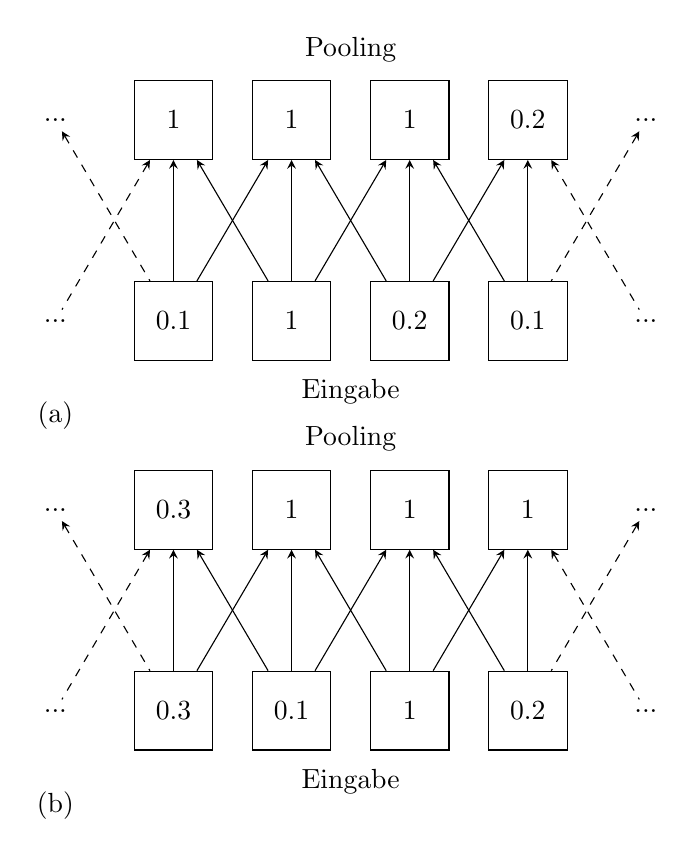
\begin{tikzpicture}[x=1.5cm, y=1.5cm, >=stealth]
			
			%\foreach \m/\l [count=\y] in {1,2,3,4}
			%\draw[gray,fill=gray](0+\y,2.5)circle(14pt);
			
			%\foreach \m/\l [count=\y] in {2,3,4}
			%\draw[gray,fill=gray](0+\m,-0.8)circle(14pt);
			
			%\draw[gray,fill=gray](3,0.8)circle(14pt);
			%\draw[gray,fill=gray](3,-2.5)circle(14pt);
			
			\foreach \m/\l [count=\y] in {1,2,3,4}
			\node [every neuron/.try, neuron \m/.try] (eins-\m) at (0+\y,2.5) {};
			
			\foreach \m/\l [count=\y] in {1,2,3,4}
			\node [every neuron/.try, neuron \m/.try] (zwei-\m) at (0+\y,0.8) {};
			
			\foreach \m/\l [count=\y] in {1,2,3,4}
			\node [every neuron/.try, neuron \m/.try] (drei-\m) at (0+\y,-0.8) {};
			
			\foreach \m/\l [count=\y] in {1,2,3,4}
			\node [every neuron/.try, neuron \m/.try] (vier-\m) at (0+\y,-2.5) {};
			
			
%			\foreach \m [count=\x] in {1,2,3,4}
%			\foreach \l [count=\i] in {1,2,3,4}
%			\draw [<-] (eins-\i) -- (zwei-\x)
%			node [] {};
			
			\node[] (1) at (1,2.5){$1$};
			\node[] (1) at (2,2.5){$1$};
			\node[] (1) at (3,2.5){$1$};
			\node[] (1) at (4,2.5){$0.2$};
			
			\node[] (1) at (1,0.8){$0.1$};
			\node[] (1) at (2,0.8){$1$};
			\node[] (1) at (3,0.8){$0.2$};
			\node[] (1) at (4,0.8){$0.1$};
			
			\node[] (1) at (1,-0.8){$0.3$};
			\node[] (1) at (2,-0.8){$1$};
			\node[] (1) at (3,-0.8){$1$};
			\node[] (1) at (4,-0.8){$1$};
			
			\node[] (1) at (1,-2.5){$0.3$};
			\node[] (1) at (2,-2.5){$0.1$};
			\node[] (1) at (3,-2.5){$1$};
			\node[] (1) at (4,-2.5){$0.2$};
			
			\node[] (1) at (2.5,3.1){Pooling};
			\node[] (1) at (2.5,0.2){Eingabe};
			\node[] (1) at (2.5,-0.2){Pooling};
			\node[] (1) at (2.5,-3.1){Eingabe};
			
			\node[] (S1) at (5,2.5){...};
			\node[] (S2) at (0,2.5){...};
			\node[] (S3) at (5,0.8){...};
			\node[] (S4) at (0,0.8){...};
			\node[] (S5) at (5,-0.8){...};
			\node[] (S6) at (0,-0.8){...};
			\node[] (S7) at (5,-2.5){...};
			\node[] (S8) at (0,-2.5){...};
			\draw [<-] (eins-1) -- (zwei-1);
			\draw [<-] (eins-1) -- (zwei-2);
			\draw [<-] (eins-2) -- (zwei-1);
			\draw [<-] (eins-2) -- (zwei-2);
			\draw [<-] (eins-2) -- (zwei-3);
			\draw [<-] (eins-3) -- (zwei-2);
			\draw [<-] (eins-3) -- (zwei-3);
			\draw [<-] (eins-3) -- (zwei-4);
			\draw [<-] (eins-4) -- (zwei-3);
			\draw [<-] (eins-4) -- (zwei-4);
			\draw [<-,dashed] (S1) -- (zwei-4);
			\draw [<-,dashed] (S2) -- (zwei-1);
			\draw [<-,dashed] (eins-1) -- (S4);
			\draw [<-,dashed] (eins-4) -- (S3);
			
			\draw [<-] (drei-1) -- (vier-1);
			\draw [<-] (drei-1) -- (vier-2);
			\draw [<-] (drei-2) -- (vier-1);
			\draw [<-] (drei-2) -- (vier-2);
			\draw [<-] (drei-2) -- (vier-3);
			\draw [<-] (drei-3) -- (vier-2);
			\draw [<-] (drei-3) -- (vier-3);
			\draw [<-] (drei-3) -- (vier-4);
			\draw [<-] (drei-4) -- (vier-3);
			\draw [<-] (drei-4) -- (vier-4);
			\draw [<-,dashed] (S5) -- (vier-4);
			\draw [<-,dashed] (S6) -- (vier-1);
			\draw [<-,dashed] (drei-1) -- (S8);
			\draw [<-,dashed] (drei-4) -- (S7);
			\node[] (a) at (0,0) {(a)};
			\node[] (a) at (0,-3.3) {(b)};
			
			
			\end{tikzpicture}
			\caption{(a) Beispielhafter Poolingprozess. Die Zahlenwerte deuten Bildinformationen als Fallbeispiel an. (b) Es gelten dieselben Darstellungsprinzipien wie in Abbildung (a). Die Eingangsdaten wurden hierbei um ein Neuron nach rechts versetzt. \cite{deeplearning}}
			\label{fig: Pooling}
		\end{figure}
	
		Beim \textit{Pooling} werden die stärksten Merkmale der eingehenden Daten weitergegeben \cite{deeplearning}. Kleine Änderungen der Eingabewerte haben durch \textit{Pooling} keinen oder einen geringen Einfluss auf die Ausgabe. Ein Beispiel hierfür liefert die folgende Darstellung \ref{fig: Pooling}. Hierbei werden die stärksten Merkmale der Eingangsdaten durch das \textit{Pooling} weitergeleitet. Obwohl in der unteren Darstellung alle Eingangsdaten um eine Stelle nach rechts verschoben wurden, hält das Verfahren zwei Merkmale konstant.\\
		
		Für die Klassifikation der Bilddaten in neuronalen Netzen setzen sich die letzten Schichten meist aus einer oder mehrerer vollständig verbundenen Schichten und einer \textit{Softmax}-Schicht zusammen \cite{deeplearning}. Die vollständig verbundene Schicht gibt einen Vektor mit $K$ Elementen aus, wobei $K$ für die Anzahl der ausgegebenen Klassen steht. Eine \textit{Softmax}-Funktion repräsentiert grundlegend eine Wahrscheinlichkeitsverteilung des Eingabevektors $K$.\\ 
		
		\begin{figure}[H]
			\centering
			\begin{tikzpicture}[node distance=4em]
			\node[3d matrix] (mat1){ 
				0 & 0 & 1 & 1 & 0 & 0 & -1 & -1 & 0 & 0 \\
			};
			\node[3d matrix,above=of mat1] (mat2){ 
				0 & 0 & 1 & 1 & 0 & 0 & -1 & -1 & 0 & 0\\
				0 & 0 & -1 & -1 & 0 & 0 & 1 & 1 & 0 & 0\\
			};
			\node[3d matrix,above=of mat2] (mat3){ 
				0 & 1 & 0 & -1 & 0 \\
				0 & -1 & 0 & 1 & 0 \\
			};
			\node[3d matrix,above=of mat3] (mat4){ 0 & -4 & 0 \\};
			\node[3d matrix,above=of mat4] (mat5){ 4 & -4 \\};
			\node[3d matrix,above=of mat5] (mat6){ 0.99 & 0.01 \\};
			\node[] (S1) at (-4,0) {Eingabe};
			\node[] (S2) at (-4,1.1) {Faltung};
			\draw[dashed](S2)--(0.5,1.1);
			\node[] (S3) at (-4,3.9) {Pooling};
			\draw[dashed](S3)--(0.5,3.9);
			\node[] (S4) at (-4,6.6) {Faltung};
			\draw[dashed](S4)--(0.5,6.6);
			\node[] (S5) at (-4,8.8) {Vollständig verbundene Schicht};
			\draw[dashed](S5)--(0.5,8.8);
			\node[] (S6) at (-4,11.1) {Softmax};
			\draw[dashed](S6)--(0.5,11.1);
			\draw[-{Latex[bend]}] (mat1.east) to[out=0,in=0] 
			coordinate[near end](aux1) ([xshift=1ex]mat2-1-10.east);
			\path (aux1) node[right,above right,3d matrix]{-1 & 0 & 1\\}; 
			\draw[-{Latex[bend]}] (mat1.east) to[out=0,in=0] ([xshift=1ex]mat2-2-10.east);
			\draw[very thick,-Latex] (mat1) -- coordinate[midway,right=2em] (aux2) (mat2);
			\path (aux2) node[right,3d matrix] (mat1a){1 & 0 & -1 \\};
			\draw[very thick,-Latex] (mat2) -- (mat3);
			\draw[very thick,-Latex] (mat3) -- (mat4)
			coordinate[midway,right=1em] (aux3);
			\path (aux3) node[right,3d matrix] (mat3a){-1 & 0 & 1 \\
				1 & 0 & -1\\};
			\foreach \X in {1,2,3} {\foreach \Y in {1,2}
				{\draw[-latex] (mat4-1-\X) -- (mat5-1-\Y);}}
			\draw[very thick,-Latex] (mat5) -- (mat6);
			\end{tikzpicture}
			\caption{Fallbeispiel eines Faltungsnetzwerks. Dreidimensional dargestellte Boxen stellen Datenpunkte dar und bilden in der horizontalen Anordnung jeweils eine Schicht. Die Prozesse der Faltung und des Poolings sind beispielhaft dargestellt. Die Flussrichtung der Bildinformationen ist durch Pfeile gekennzeichnet. \cite{cnnhor}}
			\label{fig: cnn easy}		
		\end{figure}
		
		Durch die \textit{Softmax}-Schicht wird der Vektor in einem Zahlenbereich von null bis eins transformiert. Die Summe aller Elemente des Vektors ergeben eins. Jedes Element wird als Konfidenz der jeweiligen Klasse interpretiert. An dieser Stelle sind alle Daten vollständig bearbeitet und werden als Vektor aus dem CNN ausgegeben. In Abbildung \ref{fig: cnn easy} wird die Funktionsweise eines Faltungsnetzwerks anhand eines Beispiels dargestellt.\\
		
		\section{Vergleich möglicher Konvolutionsnetze}
		\label{sec: cnns}
		Die Vielfalt der Architekturen von Konvolutionsnetzwerken ist sehr breit gefächert. Jedes Netz unterscheidet sich in der jeweiligen Architektur der Schichten. Durch die Änderung verschiedener Parameter, beispielsweise bei der Faltung oder bei dem Pooling, können CNNs im Einsatz jeweils anders reagieren. Hierbei entscheidet man bei der Auswahl des Modells häufig unter den Gesichtspunkten Bearbeitungszeit, Genauigkeit und je nach Anwendungsfall ist der Speicherplatz ebenfalls relevant.\\
		
		Die \textit{Kinect}-Kameras des ALFs sind in der Lage bis zu 30 Bilder in der Sekunde aufzunehmen. Folglich wird eine Netzarchitektur verwendet, die Bilder möglichst schnell mit einer hohen Genauigkeit verarbeitet. Für eine zukünftige Auslagerung auf ein eingebettetes System ist der Speicherplatz des Netzes sowie seine Rechenzeit von Bedeutung. Für die Auswahl der für diese Masterarbeit entsprechenden Architektur werden state-of-the-art Lösungen hinzugezogen. In \textit{Canzianis} wissenschaftlichen Beitrag \cite{cnnvergleich} werden bekannte CNNs nach der Genauigkeit über die Anzahl der Rechenoperationen pro eingegebenem Bild in einem Diagramm aufgetragen. Als dritte Eigenschaft ist dort ebenfalls die Größe der Architekturen als Parameteranzahl bemessen. Die höchsten Genauigkeiten erzielten hierbei die \textit{ResNet}, \textit{Inception} und \textit{VGG} Architekturen. \textit{Canziani} veröffentlichte sein Paper im Jahr 2016. Ein Jahr später entwickelte \textit{Howard} \cite{mobilenets} die \textit{MobileNet} Architektur. Sie zeichnet sich durch die Schnelligkeit bei teilweise höherer Genauigkeit im Vergleich zu bekannten Architekturen aus. Weiterhin werden in diesem Abschnitt die gängigen Lösungen \textit{R-CNN} und \textit{SSD} als optionale Klassifikatoren präsentiert.\\
		
		\section*{VGG}
		\label{subsec: vgg}
		Die VGG-Architektur wurde im Jahr 2015 von \textit{Simonyan} und \textit{Zisserman} \cite{vgg} vorgestellt. Oft wird die Bezeichnung \textit{VGG-xx} verwendet, wobei \textit{xx} für die Anzahl der Konvolutionsschichten in Addition mit den vollständig verbundenen Schichten steht. Bei dieser Architektur werden ausschließlich sehr kleine $3 \times 3$ Filter für die Faltung verwendet \cite{vgg}. Im Gegenzug setzten die Entwickler auf eine ausgeprägte Tiefe der Netzarchitektur. In der Publikation sind Netze bis zu einer Tiefe von 19 Schichten untersucht worden \cite{vgg}. Es hat sich herausgestellt, dass die Veränderung der Tiefe eines Netzes über die Genauigkeit der Klassifikation bestimmt \cite{vgg}. So ist das Netz in der Lage sehr hohe Genauigkeiten zu erzielen. Wiederum hängt die Anzahl der Schichten direkt mit dem Speicher- und dem Rechenaufwand eines Netzes zusammen. Ein typisches \textit{VGG-16} Netz benötigt circa 530 MB wegen seiner 138 Millionen Parameter \cite{keras}.\\
		
		\section*{ResNet}
		\label{subsec: resnet}
		\textit{ResNet} steht für \textit{residual network} und wurde erstmals im Jahr 2015 durch das Paper von \textit{He} veröffentlicht \cite{resnet}. Diese Architektur fällt besonders durch Verbindungen auf, die es Bildinformationen ermöglicht Schichten zu überspringen \cite{resnet}. So sind tiefe Zwischenschichten nicht nur von der Ausgabe der vorherigen Schicht abhängig. In Abbildung \ref{fig: residual} ist eine Prinzipdarstellung der Architektur gezeigt. Hierbei wird eine allgemeine Eingabe $x$ in beliebig viele Zwischenschichten eingegeben, die eine Ausgabe $F(x)$ erzeugt. Außerdem wird $x$ durch eine Verbindung mit $F(x)$ addiert.
		
			\tikzset{%
			every neuron/.style={
				rectangle,
				draw,
				minimum size=1cm
			},
			neuron missing/.style={
				draw=none, 
				%scale=4,
				%rotate=90,
				%yshift=1,
				%text height=0.333cm,
				%execute at begin node=\color{black}$\cdots$
			},
		}
		\begin{figure}[H]
			\centering
			
			
			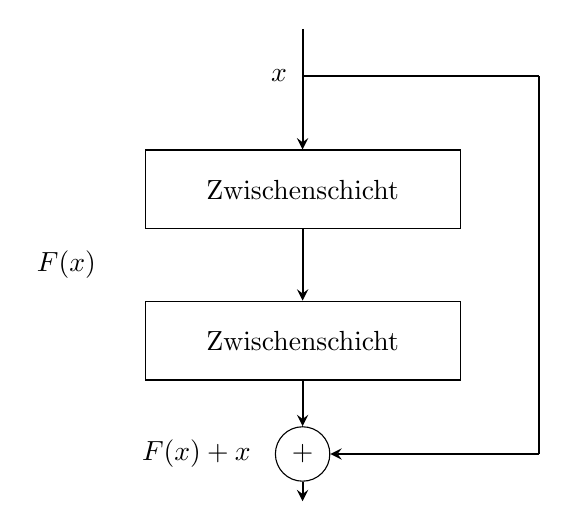
\begin{tikzpicture}[x=1.5cm, y=1.2cm, >=stealth]
			


			\node[draw,rectangle,minimum width=4cm,minimum height=1cm] (S1) at (0,-0.2) {Zwischenschicht};
			\node[draw,rectangle,minimum width=4cm,minimum height=1cm] (S2) at (0,-1.8) {Zwischenschicht};
			\node[draw,circle] (S3) at (0,-3) {+};
			\node[] (S4) at (-2,-1) {$F(x)$};
			\node[] (S4) at (-0.2,1) {$x$};
			\node[] (S4) at (-0.9,-3) {$F(x) + x$};
			\draw [->,thick]  (S1) to (S2);
			\draw [thick]  (0,1) -- (2,1);
			\draw [thick]  (2,1) to (2,-3);
			\draw [->,thick]  (2,-3) to (S3);
			\draw [->,thick]  (0,1.5) to (S1);
			\draw [->,thick]  (S2) to (S3);
			\draw [->,thick]  (S3) to (0,-3.5);
			
			
			
			\end{tikzpicture}
			\caption{Markantes Merkmal eines \textit{ResNets}. Die Flussrichtung der Bildinformationen ist als Pfeil dargestellt. Adaptiert aus \cite{resnet}}
			\label{fig: residual}
		\end{figure}
	
		\textit{ResNet} Netze erreichen je nach Größe eine höhere Genauigkeit als die bereits erwähnten \textit{VGG} Architekturen \cite{keras}. Die Größe der Netze erreichen hierbei 152 Schichten \cite{resnet}. Trotz der entsprechenden Tiefe enthält ein derartiges CNN circa die Hälfte der Parameter im Vergleich zu \textit{VGG} Netzen \cite{keras}. Dementsprechend liegt der Speicherbedarf bei circa 230 MB \cite{keras}.
		
		\section*{Inception/GoogleNet}
		\label{subsec: inception}
		Gemessen an der Top-1 Genauigkeit liegen \textit{Inception/GoogLeNet} Netze höher als \textit{VGG} und \textit{ResNet} Architekturen \cite{cnnvergleich}. \textit{Szegedy} erklärt die erste Version der \textit{Inception} CNNs in seiner Publikation \cite{inception} aus dem Jahr 2015. Die Besonderheit hierbei ist der Einsatz von multiplen Kernel auf die jeweiligen Schichten \cite{inception}. Durch diesen Aufbau benötigt ein solches Netz keine vollständig verbundene Schicht zur Klassikation, da die Genauigkeit nur geringfügig beeinträchtigt wird \cite{inception}. Gleichzeitig erfolgt eine Einsparung eines Großteils der Parameter \cite{inception}. Bei \textit{VGG} Architekturen befinden sich beispielsweise circa 90\percent\text{ }aller Parameter in den vollständig verbundenen Schichten am Ende des Netzes. Die klassische \textit{Inception} Architektur enthält insgesamt 27 Schichten, 22 davon enthalten Parameter \cite{inception}. Übliche \textit{Inception} Netze sind circa 90 MB groß und verfügen über 23 Millionen Parameter \cite{keras}.\\ 
		

		
		\section*{MobileNet}
		\label{subsec: mobilenets}
		Zu den bekanntesten state-of-the-art Lösungen gehört die \textit{MobileNet} Architektur aus dem Jahr 2017. \textit{Howard} beschreibt in seiner Paper die hohe Effizienz des Netzes hinsichtlich des Zusammenspiels zwischen Geschwindigkeit und Genauigkeit \cite{mobilenets}. Anders als bei den bisher genannten Methoden besitzen einige Kernel der Konvolutionsschichten eine dritte Dimension \cite{mobilenets}. Diese sind somit in der Lage tiefenorientierte Faltungsprozesse durchzuführen. Weiterhin wird der Rechenaufwand durch sogenannte Weiten- und Auflösungsmultiplikatoren reduziert \cite{mobilenets}. In diesem Abschnitt wird näher auf die Funktionsweise eines \textit{MobileNet} CNNs eingegangen.\\
		
		
		
		
\begin{figure}[H]
			\centering		
			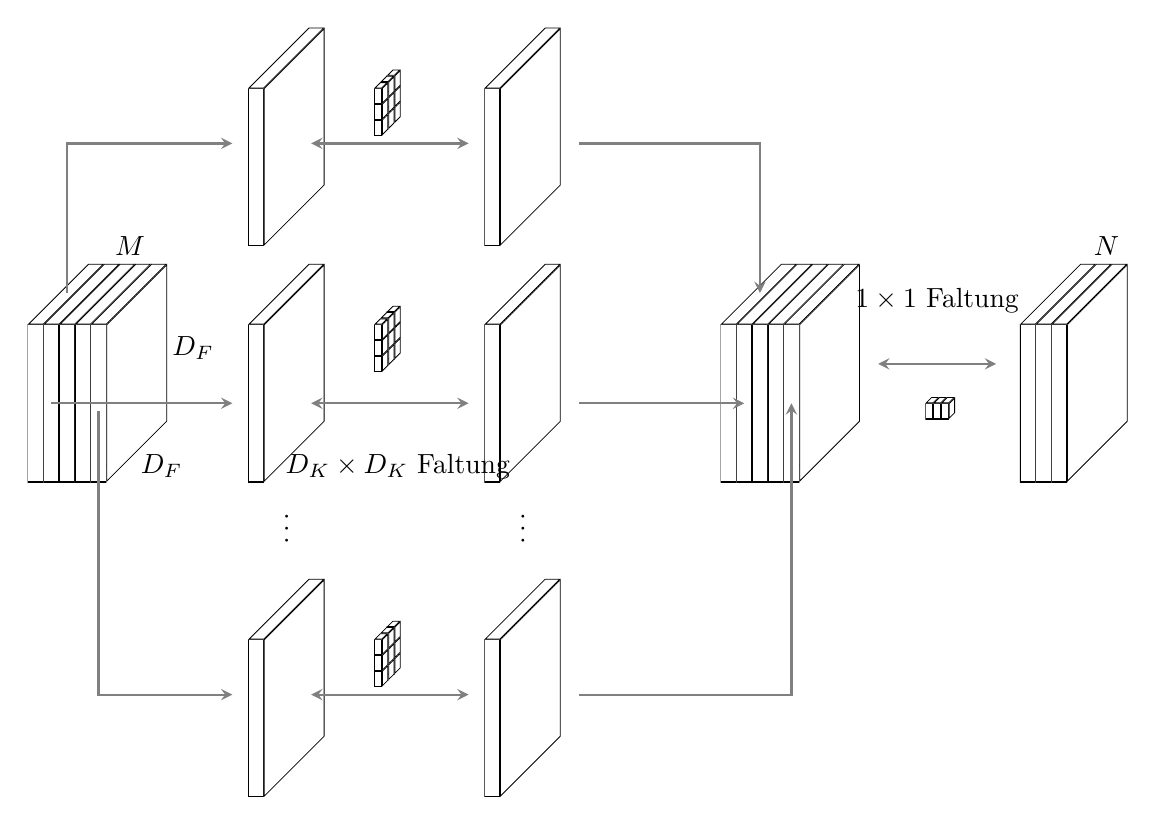
\begin{tikzpicture}
				\pgfmathsetmacro{\cubex}{0.2}
				\pgfmathsetmacro{\cubey}{2}
				\pgfmathsetmacro{\cubez}{2}
				
				\begin{scope}[yshift=-2cm,line width=0.2mm]
				\begin{scope}
				\clip[] (-0.8,0,0) -- ++(-\cubex,0,0) -- ++(0,-\cubey,0) -- ++(\cubex,0,0) -- cycle;
				\draw[fill=white] (-0.8,0,0) -- ++(-\cubex,0,0) -- ++(0,-\cubey,0) -- ++(\cubex,0,0) -- cycle;
				\end{scope}
				\begin{scope}
				\clip[] (-0.8,0,0) -- ++(0,0,-\cubez) -- ++(0,-\cubey,0) -- ++(0,0,\cubez) -- cycle;
				\draw[fill=white] (-0.8,0,0) -- ++(0,0,-\cubez) -- ++(0,-\cubey,0) -- ++(0,0,\cubez) -- cycle;
				\end{scope}
				\begin{scope}
				\clip[] (-0.8,0,0) -- ++(-\cubex,0,0) -- ++(0,0,-\cubez) -- ++(\cubex,0,0) -- cycle;
				\draw[fill=white] (-0.8,0,0) -- ++(-\cubex,0,0) -- ++(0,0,-\cubez) -- ++(\cubex,0,0) -- cycle;
				\end{scope}
				
				\begin{scope}
				\clip[] (-0.6,0,0) -- ++(-\cubex,0,0) -- ++(0,-\cubey,0) -- ++(\cubex,0,0) -- cycle;
				\draw[fill=white] (-0.6,0,0) -- ++(-\cubex,0,0) -- ++(0,-\cubey,0) -- ++(\cubex,0,0) -- cycle;
				\end{scope}
				\begin{scope}
				\clip[] (-0.6,0,0) -- ++(0,0,-\cubez) -- ++(0,-\cubey,0) -- ++(0,0,\cubez) -- cycle;
				\draw[fill=white] (-0.6,0,0) -- ++(0,0,-\cubez) -- ++(0,-\cubey,0) -- ++(0,0,\cubez) -- cycle;
				\end{scope}
				\begin{scope}
				\clip[] (-0.6,0,0) -- ++(-\cubex,0,0) -- ++(0,0,-\cubez) -- ++(\cubex,0,0) -- cycle;
				\draw[fill=white] (-0.6,0,0) -- ++(-\cubex,0,0) -- ++(0,0,-\cubez) -- ++(\cubex,0,0) -- cycle;
				\end{scope}
				
				\begin{scope}
				\clip[] (-0.4,0,0) -- ++(-\cubex,0,0) -- ++(0,-\cubey,0) -- ++(\cubex,0,0) -- cycle;
				\draw[fill=white] (-0.4,0,0) -- ++(-\cubex,0,0) -- ++(0,-\cubey,0) -- ++(\cubex,0,0) -- cycle;
				\end{scope}
				\begin{scope}
				\clip[] (-0.4,0,0) -- ++(0,0,-\cubez) -- ++(0,-\cubey,0) -- ++(0,0,\cubez) -- cycle;
				\draw[fill=white] (-0.4,0,0) -- ++(0,0,-\cubez) -- ++(0,-\cubey,0) -- ++(0,0,\cubez) -- cycle;
				\end{scope}
				\begin{scope}
				\clip[] (-0.4,0,0) -- ++(-\cubex,0,0) -- ++(0,0,-\cubez) -- ++(\cubex,0,0) -- cycle;
				\draw[fill=white] (-0.4,0,0) -- ++(-\cubex,0,0) -- ++(0,0,-\cubez) -- ++(\cubex,0,0) -- cycle;
				\end{scope}
				
				\begin{scope}
				\clip[] (-0.2,0,0) -- ++(-\cubex,0,0) -- ++(0,-\cubey,0) -- ++(\cubex,0,0) -- cycle;
				\draw[fill=white] (-0.2,0,0) -- ++(-\cubex,0,0) -- ++(0,-\cubey,0) -- ++(\cubex,0,0) -- cycle;
				\end{scope}
				\begin{scope}
				\clip[] (-0.2,0,0) -- ++(0,0,-\cubez) -- ++(0,-\cubey,0) -- ++(0,0,\cubez) -- cycle;
				\draw[fill=white] (-0.2,0,0) -- ++(0,0,-\cubez) -- ++(0,-\cubey,0) -- ++(0,0,\cubez) -- cycle;
				\end{scope}
				\begin{scope}
				\clip[] (-0.2,0,0) -- ++(-\cubex,0,0) -- ++(0,0,-\cubez) -- ++(\cubex,0,0) -- cycle;
				\draw[fill=white] (-0.2,0,0) -- ++(-\cubex,0,0) -- ++(0,0,-\cubez) -- ++(\cubex,0,0) -- cycle;
				\end{scope}
				
				\begin{scope}
				\clip[] (0,0,0) -- ++(-\cubex,0,0) -- ++(0,-\cubey,0) -- ++(\cubex,0,0) -- cycle;
				\draw[fill=white] (0,0,0) -- ++(-\cubex,0,0) -- ++(0,-\cubey,0) -- ++(\cubex,0,0) -- cycle;
				\end{scope}
				\begin{scope}
				\clip[] (0,0,0) -- ++(0,0,-\cubez) -- ++(0,-\cubey,0) -- ++(0,0,\cubez) -- cycle;
				\draw[fill=white] (0,0,0) -- ++(0,0,-\cubez) -- ++(0,-\cubey,0) -- ++(0,0,\cubez) -- cycle;
				\end{scope}
				\begin{scope}
				\clip[] (0,0,0) -- ++(-\cubex,0,0) -- ++(0,0,-\cubez) -- ++(\cubex,0,0) -- cycle;
				\draw[fill=white] (0,0,0) -- ++(-\cubex,0,0) -- ++(0,0,-\cubez) -- ++(\cubex,0,0) -- cycle;
				\end{scope}
				
				\begin{scope}
				\clip[] (2,3,0) -- ++(-\cubex,0,0) -- ++(0,-\cubey,0) -- ++(\cubex,0,0) -- cycle;
				\draw[fill=white] (2,3,0) -- ++(-\cubex,0,0) -- ++(0,-\cubey,0) -- ++(\cubex,0,0) -- cycle;
				\end{scope}
				\begin{scope}
				\clip[] (2,3,0) -- ++(0,0,-\cubez) -- ++(0,-\cubey,0) -- ++(0,0,\cubez) -- cycle;
				\draw[fill=white] (2,3,0) -- ++(0,0,-\cubez) -- ++(0,-\cubey,0) -- ++(0,0,\cubez) -- cycle;
				\end{scope}
				\begin{scope}
				\clip[] (2,3,0) -- ++(-\cubex,0,0) -- ++(0,0,-\cubez) -- ++(\cubex,0,0) -- cycle;
				\draw[fill=white] (2,3,0) -- ++(-\cubex,0,0) -- ++(0,0,-\cubez) -- ++(\cubex,0,0) -- cycle;
				\end{scope}
				
				\begin{scope}
				\clip[] (2,0,0) -- ++(-\cubex,0,0) -- ++(0,-\cubey,0) -- ++(\cubex,0,0) -- cycle;
				\draw[fill=white] (2,0,0) -- ++(-\cubex,0,0) -- ++(0,-\cubey,0) -- ++(\cubex,0,0) -- cycle;
				\end{scope}
				\begin{scope}
				\clip[] (2,0,0) -- ++(0,0,-\cubez) -- ++(0,-\cubey,0) -- ++(0,0,\cubez) -- cycle;
				\draw[fill=white] (2,0,0) -- ++(0,0,-\cubez) -- ++(0,-\cubey,0) -- ++(0,0,\cubez) -- cycle;
				\end{scope}
				\begin{scope}
				\clip[] (2,0,0) -- ++(-\cubex,0,0) -- ++(0,0,-\cubez) -- ++(\cubex,0,0) -- cycle;
				\draw[fill=white] (2,0,0) -- ++(-\cubex,0,0) -- ++(0,0,-\cubez) -- ++(\cubex,0,0) -- cycle;
				\end{scope}
				
				\begin{scope}
				\clip[] (2,-4,0) -- ++(-\cubex,0,0) -- ++(0,-\cubey,0) -- ++(\cubex,0,0) -- cycle;
				\draw[fill=white] (2,-4,0) -- ++(-\cubex,0,0) -- ++(0,-\cubey,0) -- ++(\cubex,0,0) -- cycle;
				\end{scope}
				\begin{scope}
				\clip[] (2,-4,0) -- ++(0,0,-\cubez) -- ++(0,-\cubey,0) -- ++(0,0,\cubez) -- cycle;
				\draw[fill=white] (2,-4,0) -- ++(0,0,-\cubez) -- ++(0,-\cubey,0) -- ++(0,0,\cubez) -- cycle;
				\end{scope}
				\begin{scope}
				\clip[] (2,-4,0) -- ++(-\cubex,0,0) -- ++(0,0,-\cubez) -- ++(\cubex,0,0) -- cycle;
				\draw[fill=white] (2,-4,0) -- ++(-\cubex,0,0) -- ++(0,0,-\cubez) -- ++(\cubex,0,0) -- cycle;
				\end{scope}
				
				\begin{scope}
				\clip[] (5,3,0) -- ++(-\cubex,0,0) -- ++(0,-\cubey,0) -- ++(\cubex,0,0) -- cycle;
				\draw[fill=white] (5,3,0) -- ++(-\cubex,0,0) -- ++(0,-\cubey,0) -- ++(\cubex,0,0) -- cycle;
				\end{scope}
				\begin{scope}
				\clip[] (5,3,0) -- ++(0,0,-\cubez) -- ++(0,-\cubey,0) -- ++(0,0,\cubez) -- cycle;
				\draw[fill=white] (5,3,0) -- ++(0,0,-\cubez) -- ++(0,-\cubey,0) -- ++(0,0,\cubez) -- cycle;
				\end{scope}
				\begin{scope}
				\clip[] (5,3,0) -- ++(-\cubex,0,0) -- ++(0,0,-\cubez) -- ++(\cubex,0,0) -- cycle;
				\draw[fill=white] (5,3,0) -- ++(-\cubex,0,0) -- ++(0,0,-\cubez) -- ++(\cubex,0,0) -- cycle;
				\end{scope}
				
				\begin{scope}
				\clip[] (5,0,0) -- ++(-\cubex,0,0) -- ++(0,-\cubey,0) -- ++(\cubex,0,0) -- cycle;
				\draw[fill=white] (5,0,0) -- ++(-\cubex,0,0) -- ++(0,-\cubey,0) -- ++(\cubex,0,0) -- cycle;
				\end{scope}
				\begin{scope}
				\clip[] (5,0,0) -- ++(0,0,-\cubez) -- ++(0,-\cubey,0) -- ++(0,0,\cubez) -- cycle;
				\draw[fill=white] (5,0,0) -- ++(0,0,-\cubez) -- ++(0,-\cubey,0) -- ++(0,0,\cubez) -- cycle;
				\end{scope}
				\begin{scope}
				\clip[] (5,0,0) -- ++(-\cubex,0,0) -- ++(0,0,-\cubez) -- ++(\cubex,0,0) -- cycle;
				\draw[fill=white] (5,0,0) -- ++(-\cubex,0,0) -- ++(0,0,-\cubez) -- ++(\cubex,0,0) -- cycle;
				\end{scope}
				
				%untere Platte rechts
				\begin{scope}
				\clip[] (5,-4,0) -- ++(-\cubex,0,0) -- ++(0,-\cubey,0) -- ++(\cubex,0,0) -- cycle;
				\draw[fill=white] (5,-4,0) -- ++(-\cubex,0,0) -- ++(0,-\cubey,0) -- ++(\cubex,0,0) -- cycle;
				\end{scope}
				\begin{scope}
				\clip[] (5,-4,0) -- ++(0,0,-\cubez) -- ++(0,-\cubey,0) -- ++(0,0,\cubez) -- cycle;
				\draw[fill=white] (5,-4,0) -- ++(0,0,-\cubez) -- ++(0,-\cubey,0) -- ++(0,0,\cubez) -- cycle;
				\end{scope}
				\begin{scope}
				\clip[] (5,-4,0) -- ++(-\cubex,0,0) -- ++(0,0,-\cubez) -- ++(\cubex,0,0) -- cycle;
				\draw[fill=white] (5,-4,0) -- ++(-\cubex,0,0) -- ++(0,0,-\cubez) -- ++(\cubex,0,0) -- cycle;
				\end{scope}
			
				%rechtes Fünferpack
				\begin{scope}
				\clip[] (8,0,0) -- ++(-\cubex,0,0) -- ++(0,-\cubey,0) -- ++(\cubex,0,0) -- cycle;
				\draw[fill=white] (8,0,0) -- ++(-\cubex,0,0) -- ++(0,-\cubey,0) -- ++(\cubex,0,0) -- cycle;
				\end{scope}
				\begin{scope}
				\clip[] (8,0,0) -- ++(0,0,-\cubez) -- ++(0,-\cubey,0) -- ++(0,0,\cubez) -- cycle;
				\draw[fill=white] (8,0,0) -- ++(0,0,-\cubez) -- ++(0,-\cubey,0) -- ++(0,0,\cubez) -- cycle;
				\end{scope}
				\begin{scope}
				\clip[] (8,0,0) -- ++(-\cubex,0,0) -- ++(0,0,-\cubez) -- ++(\cubex,0,0) -- cycle;
				\draw[fill=white] (8,0,0) -- ++(-\cubex,0,0) -- ++(0,0,-\cubez) -- ++(\cubex,0,0) -- cycle;
				\end{scope}
				
				\begin{scope}
				\clip[] (8.2,0,0) -- ++(-\cubex,0,0) -- ++(0,-\cubey,0) -- ++(\cubex,0,0) -- cycle;
				\draw[fill=white] (8.2,0,0) -- ++(-\cubex,0,0) -- ++(0,-\cubey,0) -- ++(\cubex,0,0) -- cycle;
				\end{scope}
				\begin{scope}
				\clip[] (8.2,0,0) -- ++(0,0,-\cubez) -- ++(0,-\cubey,0) -- ++(0,0,\cubez) -- cycle;
				\draw[fill=white] (8.2,0,0) -- ++(0,0,-\cubez) -- ++(0,-\cubey,0) -- ++(0,0,\cubez) -- cycle;
				\end{scope}
				\begin{scope}
				\clip[] (8.2,0,0) -- ++(-\cubex,0,0) -- ++(0,0,-\cubez) -- ++(\cubex,0,0) -- cycle;
				\draw[fill=white] (8.2,0,0) -- ++(-\cubex,0,0) -- ++(0,0,-\cubez) -- ++(\cubex,0,0) -- cycle;
				\end{scope}
				
				\begin{scope}
				\clip[] (8.4,0,0) -- ++(-\cubex,0,0) -- ++(0,-\cubey,0) -- ++(\cubex,0,0) -- cycle;
				\draw[fill=white] (8.4,0,0) -- ++(-\cubex,0,0) -- ++(0,-\cubey,0) -- ++(\cubex,0,0) -- cycle;
				\end{scope}
				\begin{scope}
				\clip[] (8.4,0,0) -- ++(0,0,-\cubez) -- ++(0,-\cubey,0) -- ++(0,0,\cubez) -- cycle;
				\draw[fill=white] (8.4,0,0) -- ++(0,0,-\cubez) -- ++(0,-\cubey,0) -- ++(0,0,\cubez) -- cycle;
				\end{scope}
				\begin{scope}
				\clip[] (8.4,0,0) -- ++(-\cubex,0,0) -- ++(0,0,-\cubez) -- ++(\cubex,0,0) -- cycle;
				\draw[fill=white] (8.4,0,0) -- ++(-\cubex,0,0) -- ++(0,0,-\cubez) -- ++(\cubex,0,0) -- cycle;
				\end{scope}
				
				\begin{scope}
				\clip[] (8.6,0,0) -- ++(-\cubex,0,0) -- ++(0,-\cubey,0) -- ++(\cubex,0,0) -- cycle;
				\draw[fill=white] (8.6,0,0) -- ++(-\cubex,0,0) -- ++(0,-\cubey,0) -- ++(\cubex,0,0) -- cycle;
				\end{scope}
				\begin{scope}
				\clip[] (8.6,0,0) -- ++(0,0,-\cubez) -- ++(0,-\cubey,0) -- ++(0,0,\cubez) -- cycle;
				\draw[fill=white] (8.6,0,0) -- ++(0,0,-\cubez) -- ++(0,-\cubey,0) -- ++(0,0,\cubez) -- cycle;
				\end{scope}
				\begin{scope}
				\clip[] (8.6,0,0) -- ++(-\cubex,0,0) -- ++(0,0,-\cubez) -- ++(\cubex,0,0) -- cycle;
				\draw[fill=white] (8.6,0,0) -- ++(-\cubex,0,0) -- ++(0,0,-\cubez) -- ++(\cubex,0,0) -- cycle;
				\end{scope}
				
				\begin{scope}
				\clip[] (8.8,0,0) -- ++(-\cubex,0,0) -- ++(0,-\cubey,0) -- ++(\cubex,0,0) -- cycle;
				\draw[fill=white] (8.8,0,0) -- ++(-\cubex,0,0) -- ++(0,-\cubey,0) -- ++(\cubex,0,0) -- cycle;
				\end{scope}
				\begin{scope}
				\clip[] (8.8,0,0) -- ++(0,0,-\cubez) -- ++(0,-\cubey,0) -- ++(0,0,\cubez) -- cycle;
				\draw[fill=white] (8.8,0,0) -- ++(0,0,-\cubez) -- ++(0,-\cubey,0) -- ++(0,0,\cubez) -- cycle;
				\end{scope}
				\begin{scope}
				\clip[] (8.8,0,0) -- ++(-\cubex,0,0) -- ++(0,0,-\cubez) -- ++(\cubex,0,0) -- cycle;
				\draw[fill=white] (8.8,0,0) -- ++(-\cubex,0,0) -- ++(0,0,-\cubez) -- ++(\cubex,0,0) -- cycle;
				\end{scope}
			
				%Dreierpack
				\begin{scope}
				\clip[] (11.8,0,0) -- ++(-\cubex,0,0) -- ++(0,-\cubey,0) -- ++(\cubex,0,0) -- cycle;
				\draw[fill=white] (11.8,0,0) -- ++(-\cubex,0,0) -- ++(0,-\cubey,0) -- ++(\cubex,0,0) -- cycle;
				\end{scope}
				\begin{scope}
				\clip[] (11.8,0,0) -- ++(0,0,-\cubez) -- ++(0,-\cubey,0) -- ++(0,0,\cubez) -- cycle;
				\draw[fill=white] (11.8,0,0) -- ++(0,0,-\cubez) -- ++(0,-\cubey,0) -- ++(0,0,\cubez) -- cycle;
				\end{scope}
				\begin{scope}
				\clip[] (11.8,0,0) -- ++(-\cubex,0,0) -- ++(0,0,-\cubez) -- ++(\cubex,0,0) -- cycle;
				\draw[fill=white] (11.8,0,0) -- ++(-\cubex,0,0) -- ++(0,0,-\cubez) -- ++(\cubex,0,0) -- cycle;
				\end{scope}
				
				\begin{scope}
				\clip[] (12,0,0) -- ++(-\cubex,0,0) -- ++(0,-\cubey,0) -- ++(\cubex,0,0) -- cycle;
				\draw[fill=white] (12,0,0) -- ++(-\cubex,0,0) -- ++(0,-\cubey,0) -- ++(\cubex,0,0) -- cycle;
				\end{scope}
				\begin{scope}
				\clip[] (12,0,0) -- ++(0,0,-\cubez) -- ++(0,-\cubey,0) -- ++(0,0,\cubez) -- cycle;
				\draw[fill=white] (12,0,0) -- ++(0,0,-\cubez) -- ++(0,-\cubey,0) -- ++(0,0,\cubez) -- cycle;
				\end{scope}
				\begin{scope}
				\clip[] (12,0,0) -- ++(-\cubex,0,0) -- ++(0,0,-\cubez) -- ++(\cubex,0,0) -- cycle;
				\draw[fill=white] (12,0,0) -- ++(-\cubex,0,0) -- ++(0,0,-\cubez) -- ++(\cubex,0,0) -- cycle;
				\end{scope}
				
				\begin{scope}
				\clip[] (12.2,0,0) -- ++(-\cubex,0,0) -- ++(0,-\cubey,0) -- ++(\cubex,0,0) -- cycle;
				\draw[fill=white] (12.2,0,0) -- ++(-\cubex,0,0) -- ++(0,-\cubey,0) -- ++(\cubex,0,0) -- cycle;
				\end{scope}
				\begin{scope}
				\clip[] (12.2,0,0) -- ++(0,0,-\cubez) -- ++(0,-\cubey,0) -- ++(0,0,\cubez) -- cycle;
				\draw[fill=white] (12.2,0,0) -- ++(0,0,-\cubez) -- ++(0,-\cubey,0) -- ++(0,0,\cubez) -- cycle;
				\end{scope}
				\begin{scope}
				\clip[] (12.2,0,0) -- ++(-\cubex,0,0) -- ++(0,0,-\cubez) -- ++(\cubex,0,0) -- cycle;
				\draw[fill=white] (12.2,0,0) -- ++(-\cubex,0,0) -- ++(0,0,-\cubez) -- ++(\cubex,0,0) -- cycle;
				\end{scope}
				
				\pgfmathsetmacro{\cubex}{0.1}
				\pgfmathsetmacro{\cubey}{0.2}
				\pgfmathsetmacro{\cubez}{0.2}
				
					%Filter oben
				\begin{scope}
					\clip[] (3.66,2.76,0) -- ++(-\cubex,0,0) -- ++(0,-\cubey,0) -- ++(\cubex,0,0) -- cycle;
					\draw[fill=white] (3.66,2.76,0) -- ++(-\cubex,0,0) -- ++(0,-\cubey,0) -- ++(\cubex,0,0) -- cycle;
				\end{scope}
				\begin{scope}
					\clip[] (3.66,2.76,0) -- ++(0,0,-\cubez) -- ++(0,-\cubey,0) -- ++(0,0,\cubez) -- cycle;
					\draw[fill=white] (3.66,2.76,0) -- ++(0,0,-\cubez) -- ++(0,-\cubey,0) -- ++(0,0,\cubez) -- cycle;
				\end{scope}
				\begin{scope}
					\clip[] (3.66,2.76,0) -- ++(-\cubex,0,0) -- ++(0,0,-\cubez) -- ++(\cubex,0,0) -- cycle;
					\draw[fill=white] (3.66,2.76,0) -- ++(-\cubex,0,0) -- ++(0,0,-\cubez) -- ++(\cubex,0,0) -- cycle;
				\end{scope}
				
				\begin{scope}
					\clip[] (3.58,2.68,0) -- ++(-\cubex,0,0) -- ++(0,-\cubey,0) -- ++(\cubex,0,0) -- cycle;
					\draw[fill=white] (3.58,2.68,0) -- ++(-\cubex,0,0) -- ++(0,-\cubey,0) -- ++(\cubex,0,0) -- cycle;
				\end{scope}
				\begin{scope}
					\clip[] (3.58,2.68,0) -- ++(0,0,-\cubez) -- ++(0,-\cubey,0) -- ++(0,0,\cubez) -- cycle;
					\draw[fill=white] (3.58,2.68,0) -- ++(0,0,-\cubez) -- ++(0,-\cubey,0) -- ++(0,0,\cubez) -- cycle;
				\end{scope}
				\begin{scope}
					\clip[] (3.58,2.68,0) -- ++(-\cubex,0,0) -- ++(0,0,-\cubez) -- ++(\cubex,0,0) -- cycle;
					\draw[fill=white] (3.58,2.68,0) -- ++(-\cubex,0,0) -- ++(0,0,-\cubez) -- ++(\cubex,0,0) -- cycle;
				\end{scope}
				
				\begin{scope}
					\clip[] (3.5,2.6,0) -- ++(-\cubex,0,0) -- ++(0,-\cubey,0) -- ++(\cubex,0,0) -- cycle;
					\draw[fill=white] (3.5,2.6,0) -- ++(-\cubex,0,0) -- ++(0,-\cubey,0) -- ++(\cubex,0,0) -- cycle;
				\end{scope}
				\begin{scope}
					\clip[] (3.5,2.6,0) -- ++(0,0,-\cubez) -- ++(0,-\cubey,0) -- ++(0,0,\cubez) -- cycle;
					\draw[fill=white] (3.5,2.6,0) -- ++(0,0,-\cubez) -- ++(0,-\cubey,0) -- ++(0,0,\cubez) -- cycle;
				\end{scope}
				\begin{scope}
					\clip[] (3.5,2.6,0) -- ++(-\cubex,0,0) -- ++(0,0,-\cubez) -- ++(\cubex,0,0) -- cycle;
					\draw[fill=white] (3.5,2.6,0) -- ++(-\cubex,0,0) -- ++(0,0,-\cubez) -- ++(\cubex,0,0) -- cycle;
				\end{scope}
				
				\begin{scope}
					\clip[] (3.66,2.96,0) -- ++(-\cubex,0,0) -- ++(0,-\cubey,0) -- ++(\cubex,0,0) -- cycle;
					\draw[fill=white] (3.66,2.96,0) -- ++(-\cubex,0,0) -- ++(0,-\cubey,0) -- ++(\cubex,0,0) -- cycle;
				\end{scope}
				\begin{scope}
					\clip[] (3.66,2.96,0) -- ++(0,0,-\cubez) -- ++(0,-\cubey,0) -- ++(0,0,\cubez) -- cycle;
					\draw[fill=white] (3.66,2.96,0) -- ++(0,0,-\cubez) -- ++(0,-\cubey,0) -- ++(0,0,\cubez) -- cycle;
				\end{scope}
				\begin{scope}
					\clip[] (3.66,2.96,0) -- ++(-\cubex,0,0) -- ++(0,0,-\cubez) -- ++(\cubex,0,0) -- cycle;
					\draw[fill=white] (3.66,2.96,0) -- ++(-\cubex,0,0) -- ++(0,0,-\cubez) -- ++(\cubex,0,0) -- cycle;
				\end{scope}
				
				\begin{scope}
					\clip[] (3.58,2.88,0) -- ++(-\cubex,0,0) -- ++(0,-\cubey,0) -- ++(\cubex,0,0) -- cycle;
					\draw[fill=white] (3.58,2.88,0) -- ++(-\cubex,0,0) -- ++(0,-\cubey,0) -- ++(\cubex,0,0) -- cycle;
				\end{scope}
				\begin{scope}
					\clip[] (3.58,2.88,0) -- ++(0,0,-\cubez) -- ++(0,-\cubey,0) -- ++(0,0,\cubez) -- cycle;
					\draw[fill=white] (3.58,2.88,0) -- ++(0,0,-\cubez) -- ++(0,-\cubey,0) -- ++(0,0,\cubez) -- cycle;
				\end{scope}
				\begin{scope}
					\clip[] (3.58,2.88,0) -- ++(-\cubex,0,0) -- ++(0,0,-\cubez) -- ++(\cubex,0,0) -- cycle;
					\draw[fill=white] (3.58,2.88,0) -- ++(-\cubex,0,0) -- ++(0,0,-\cubez) -- ++(\cubex,0,0) -- cycle;
				\end{scope}
				
				\begin{scope}
					\clip[] (3.5,2.8,0) -- ++(-\cubex,0,0) -- ++(0,-\cubey,0) -- ++(\cubex,0,0) -- cycle;
					\draw[fill=white] (3.5,2.8,0) -- ++(-\cubex,0,0) -- ++(0,-\cubey,0) -- ++(\cubex,0,0) -- cycle;
				\end{scope}
				\begin{scope}
					\clip[] (3.5,2.8,0) -- ++(0,0,-\cubez) -- ++(0,-\cubey,0) -- ++(0,0,\cubez) -- cycle;
					\draw[fill=white] (3.5,2.8,0) -- ++(0,0,-\cubez) -- ++(0,-\cubey,0) -- ++(0,0,\cubez) -- cycle;
				\end{scope}
				\begin{scope}
					\clip[] (3.5,2.8,0) -- ++(-\cubex,0,0) -- ++(0,0,-\cubez) -- ++(\cubex,0,0) -- cycle;
					\draw[fill=white] (3.5,2.8,0) -- ++(-\cubex,0,0) -- ++(0,0,-\cubez) -- ++(\cubex,0,0) -- cycle;
				\end{scope}
				
				\begin{scope}
					\clip[] (3.66,3.16,0) -- ++(-\cubex,0,0) -- ++(0,-\cubey,0) -- ++(\cubex,0,0) -- cycle;
					\draw[fill=white] (3.66,3.16,0) -- ++(-\cubex,0,0) -- ++(0,-\cubey,0) -- ++(\cubex,0,0) -- cycle;
				\end{scope}
				\begin{scope}
					\clip[] (3.66,3.16,0) -- ++(0,0,-\cubez) -- ++(0,-\cubey,0) -- ++(0,0,\cubez) -- cycle;
					\draw[fill=white] (3.66,3.16,0) -- ++(0,0,-\cubez) -- ++(0,-\cubey,0) -- ++(0,0,\cubez) -- cycle;
				\end{scope}
				\begin{scope}
					\clip[] (3.66,3.16,0) -- ++(-\cubex,0,0) -- ++(0,0,-\cubez) -- ++(\cubex,0,0) -- cycle;
					\draw[fill=white] (3.66,3.16,0) -- ++(-\cubex,0,0) -- ++(0,0,-\cubez) -- ++(\cubex,0,0) -- cycle;
				\end{scope}
				
				\begin{scope}
					\clip[] (3.58,3.08,0) -- ++(-\cubex,0,0) -- ++(0,-\cubey,0) -- ++(\cubex,0,0) -- cycle;
					\draw[fill=white] (3.58,3.08,0) -- ++(-\cubex,0,0) -- ++(0,-\cubey,0) -- ++(\cubex,0,0) -- cycle;
				\end{scope}
				\begin{scope}
					\clip[] (3.58,3.08,0) -- ++(0,0,-\cubez) -- ++(0,-\cubey,0) -- ++(0,0,\cubez) -- cycle;
					\draw[fill=white] (3.58,3.08,0) -- ++(0,0,-\cubez) -- ++(0,-\cubey,0) -- ++(0,0,\cubez) -- cycle;
				\end{scope}
				\begin{scope}
					\clip[] (3.58,3.08,0) -- ++(-\cubex,0,0) -- ++(0,0,-\cubez) -- ++(\cubex,0,0) -- cycle;
					\draw[fill=white] (3.58,3.08,0) -- ++(-\cubex,0,0) -- ++(0,0,-\cubez) -- ++(\cubex,0,0) -- cycle;
				\end{scope}
				
				\begin{scope}
					\clip[] (3.5,3,0) -- ++(-\cubex,0,0) -- ++(0,-\cubey,0) -- ++(\cubex,0,0) -- cycle;
					\draw[fill=white] (3.5,3,0) -- ++(-\cubex,0,0) -- ++(0,-\cubey,0) -- ++(\cubex,0,0) -- cycle;
				\end{scope}
				\begin{scope}
					\clip[] (3.5,3,0) -- ++(0,0,-\cubez) -- ++(0,-\cubey,0) -- ++(0,0,\cubez) -- cycle;
					\draw[fill=white] (3.5,3,0) -- ++(0,0,-\cubez) -- ++(0,-\cubey,0) -- ++(0,0,\cubez) -- cycle;
				\end{scope}
				\begin{scope}
					\clip[] (3.5,3,0) -- ++(-\cubex,0,0) -- ++(0,0,-\cubez) -- ++(\cubex,0,0) -- cycle;
					\draw[fill=white] (3.5,3,0) -- ++(-\cubex,0,0) -- ++(0,0,-\cubez) -- ++(\cubex,0,0) -- cycle;
				\end{scope}
				
				%Filter mitte
				\begin{scope}
				\clip[] (3.66,-0.24,0) -- ++(-\cubex,0,0) -- ++(0,-\cubey,0) -- ++(\cubex,0,0) -- cycle;
				\draw[fill=white] (3.66,-0.24,0) -- ++(-\cubex,0,0) -- ++(0,-\cubey,0) -- ++(\cubex,0,0) -- cycle;
				\end{scope}
				\begin{scope}
				\clip[] (3.66,-0.24,0) -- ++(0,0,-\cubez) -- ++(0,-\cubey,0) -- ++(0,0,\cubez) -- cycle;
				\draw[fill=white] (3.66,-0.24,0) -- ++(0,0,-\cubez) -- ++(0,-\cubey,0) -- ++(0,0,\cubez) -- cycle;
				\end{scope}
				\begin{scope}
				\clip[] (3.66,-0.24,0) -- ++(-\cubex,0,0) -- ++(0,0,-\cubez) -- ++(\cubex,0,0) -- cycle;
				\draw[fill=white] (3.66,-0.24,0) -- ++(-\cubex,0,0) -- ++(0,0,-\cubez) -- ++(\cubex,0,0) -- cycle;
				\end{scope}
				
				\begin{scope}
				\clip[] (3.58,-0.32,0) -- ++(-\cubex,0,0) -- ++(0,-\cubey,0) -- ++(\cubex,0,0) -- cycle;
				\draw[fill=white] (3.58,-0.32,0) -- ++(-\cubex,0,0) -- ++(0,-\cubey,0) -- ++(\cubex,0,0) -- cycle;
				\end{scope}
				\begin{scope}
				\clip[] (3.58,-0.32,0) -- ++(0,0,-\cubez) -- ++(0,-\cubey,0) -- ++(0,0,\cubez) -- cycle;
				\draw[fill=white] (3.58,-0.32,0) -- ++(0,0,-\cubez) -- ++(0,-\cubey,0) -- ++(0,0,\cubez) -- cycle;
				\end{scope}
				\begin{scope}
				\clip[] (3.58,-0.32,0) -- ++(-\cubex,0,0) -- ++(0,0,-\cubez) -- ++(\cubex,0,0) -- cycle;
				\draw[fill=white] (3.58,-0.32,0) -- ++(-\cubex,0,0) -- ++(0,0,-\cubez) -- ++(\cubex,0,0) -- cycle;
				\end{scope}
				
				\begin{scope}
				\clip[] (3.5,-0.4,0) -- ++(-\cubex,0,0) -- ++(0,-\cubey,0) -- ++(\cubex,0,0) -- cycle;
				\draw[fill=white] (3.5,-0.4,0) -- ++(-\cubex,0,0) -- ++(0,-\cubey,0) -- ++(\cubex,0,0) -- cycle;
				\end{scope}
				\begin{scope}
				\clip[] (3.5,-0.4,0) -- ++(0,0,-\cubez) -- ++(0,-\cubey,0) -- ++(0,0,\cubez) -- cycle;
				\draw[fill=white] (3.5,-0.4,0) -- ++(0,0,-\cubez) -- ++(0,-\cubey,0) -- ++(0,0,\cubez) -- cycle;
				\end{scope}
				\begin{scope}
				\clip[] (3.5,-0.4,0) -- ++(-\cubex,0,0) -- ++(0,0,-\cubez) -- ++(\cubex,0,0) -- cycle;
				\draw[fill=white] (3.5,-0.4,0) -- ++(-\cubex,0,0) -- ++(0,0,-\cubez) -- ++(\cubex,0,0) -- cycle;
				\end{scope}
				
				\begin{scope}
				\clip[] (3.66,-0.04,0) -- ++(-\cubex,0,0) -- ++(0,-\cubey,0) -- ++(\cubex,0,0) -- cycle;
				\draw[fill=white] (3.66,-0.04,0) -- ++(-\cubex,0,0) -- ++(0,-\cubey,0) -- ++(\cubex,0,0) -- cycle;
				\end{scope}
				\begin{scope}
				\clip[] (3.66,-0.04,0) -- ++(0,0,-\cubez) -- ++(0,-\cubey,0) -- ++(0,0,\cubez) -- cycle;
				\draw[fill=white] (3.66,-0.04,0) -- ++(0,0,-\cubez) -- ++(0,-\cubey,0) -- ++(0,0,\cubez) -- cycle;
				\end{scope}
				\begin{scope}
				\clip[] (3.66,-0.04,0) -- ++(-\cubex,0,0) -- ++(0,0,-\cubez) -- ++(\cubex,0,0) -- cycle;
				\draw[fill=white] (3.66,-0.04,0) -- ++(-\cubex,0,0) -- ++(0,0,-\cubez) -- ++(\cubex,0,0) -- cycle;
				\end{scope}
				
				\begin{scope}
				\clip[] (3.58,-0.12,0) -- ++(-\cubex,0,0) -- ++(0,-\cubey,0) -- ++(\cubex,0,0) -- cycle;
				\draw[fill=white] (3.58,-0.12,0) -- ++(-\cubex,0,0) -- ++(0,-\cubey,0) -- ++(\cubex,0,0) -- cycle;
				\end{scope}
				\begin{scope}
				\clip[] (3.58,-0.12,0) -- ++(0,0,-\cubez) -- ++(0,-\cubey,0) -- ++(0,0,\cubez) -- cycle;
				\draw[fill=white] (3.58,-0.12,0) -- ++(0,0,-\cubez) -- ++(0,-\cubey,0) -- ++(0,0,\cubez) -- cycle;
				\end{scope}
				\begin{scope}
				\clip[] (3.58,-0.12,0) -- ++(-\cubex,0,0) -- ++(0,0,-\cubez) -- ++(\cubex,0,0) -- cycle;
				\draw[fill=white] (3.58,-0.12,0) -- ++(-\cubex,0,0) -- ++(0,0,-\cubez) -- ++(\cubex,0,0) -- cycle;
				\end{scope}
				
				\begin{scope}
				\clip[] (3.5,-0.2,0) -- ++(-\cubex,0,0) -- ++(0,-\cubey,0) -- ++(\cubex,0,0) -- cycle;
				\draw[fill=white] (3.5,-0.2,0) -- ++(-\cubex,0,0) -- ++(0,-\cubey,0) -- ++(\cubex,0,0) -- cycle;
				\end{scope}
				\begin{scope}
				\clip[] (3.5,-0.2,0) -- ++(0,0,-\cubez) -- ++(0,-\cubey,0) -- ++(0,0,\cubez) -- cycle;
				\draw[fill=white] (3.5,-0.2,0) -- ++(0,0,-\cubez) -- ++(0,-\cubey,0) -- ++(0,0,\cubez) -- cycle;
				\end{scope}
				\begin{scope}
				\clip[] (3.5,-0.2,0) -- ++(-\cubex,0,0) -- ++(0,0,-\cubez) -- ++(\cubex,0,0) -- cycle;
				\draw[fill=white] (3.5,-0.2,0) -- ++(-\cubex,0,0) -- ++(0,0,-\cubez) -- ++(\cubex,0,0) -- cycle;
				\end{scope}
				
				\begin{scope}
				\clip[] (3.66,0.16,0) -- ++(-\cubex,0,0) -- ++(0,-\cubey,0) -- ++(\cubex,0,0) -- cycle;
				\draw[fill=white] (3.66,0.16,0) -- ++(-\cubex,0,0) -- ++(0,-\cubey,0) -- ++(\cubex,0,0) -- cycle;
				\end{scope}
				\begin{scope}
				\clip[] (3.66,0.16,0) -- ++(0,0,-\cubez) -- ++(0,-\cubey,0) -- ++(0,0,\cubez) -- cycle;
				\draw[fill=white] (3.66,0.16,0) -- ++(0,0,-\cubez) -- ++(0,-\cubey,0) -- ++(0,0,\cubez) -- cycle;
				\end{scope}
				\begin{scope}
				\clip[] (3.66,0.16,0) -- ++(-\cubex,0,0) -- ++(0,0,-\cubez) -- ++(\cubex,0,0) -- cycle;
				\draw[fill=white] (3.66,0.16,0) -- ++(-\cubex,0,0) -- ++(0,0,-\cubez) -- ++(\cubex,0,0) -- cycle;
				\end{scope}
				
				\begin{scope}
				\clip[] (3.58,0.08,0) -- ++(-\cubex,0,0) -- ++(0,-\cubey,0) -- ++(\cubex,0,0) -- cycle;
				\draw[fill=white] (3.58,0.08,0) -- ++(-\cubex,0,0) -- ++(0,-\cubey,0) -- ++(\cubex,0,0) -- cycle;
				\end{scope}
				\begin{scope}
				\clip[] (3.58,0.08,0) -- ++(0,0,-\cubez) -- ++(0,-\cubey,0) -- ++(0,0,\cubez) -- cycle;
				\draw[fill=white] (3.58,0.08,0) -- ++(0,0,-\cubez) -- ++(0,-\cubey,0) -- ++(0,0,\cubez) -- cycle;
				\end{scope}
				\begin{scope}
				\clip[] (3.58,0.08,0) -- ++(-\cubex,0,0) -- ++(0,0,-\cubez) -- ++(\cubex,0,0) -- cycle;
				\draw[fill=white] (3.58,0.08,0) -- ++(-\cubex,0,0) -- ++(0,0,-\cubez) -- ++(\cubex,0,0) -- cycle;
				\end{scope}
				
				\begin{scope}
				\clip[] (3.5,0,0) -- ++(-\cubex,0,0) -- ++(0,-\cubey,0) -- ++(\cubex,0,0) -- cycle;
				\draw[fill=white] (3.5,0,0) -- ++(-\cubex,0,0) -- ++(0,-\cubey,0) -- ++(\cubex,0,0) -- cycle;
				\end{scope}
				\begin{scope}
				\clip[] (3.5,0,0) -- ++(0,0,-\cubez) -- ++(0,-\cubey,0) -- ++(0,0,\cubez) -- cycle;
				\draw[fill=white] (3.5,0,0) -- ++(0,0,-\cubez) -- ++(0,-\cubey,0) -- ++(0,0,\cubez) -- cycle;
				\end{scope}
				\begin{scope}
				\clip[] (3.5,0,0) -- ++(-\cubex,0,0) -- ++(0,0,-\cubez) -- ++(\cubex,0,0) -- cycle;
				\draw[fill=white] (3.5,0,0) -- ++(-\cubex,0,0) -- ++(0,0,-\cubez) -- ++(\cubex,0,0) -- cycle;
				\end{scope}
			
				%Filter unten
				\begin{scope}
					\clip[] (3.66,-4.24,0) -- ++(-\cubex,0,0) -- ++(0,-\cubey,0) -- ++(\cubex,0,0) -- cycle;
					\draw[fill=white] (3.66,-4.24,0) -- ++(-\cubex,0,0) -- ++(0,-\cubey,0) -- ++(\cubex,0,0) -- cycle;
				\end{scope}
				\begin{scope}
					\clip[] (3.66,-4.24,0) -- ++(0,0,-\cubez) -- ++(0,-\cubey,0) -- ++(0,0,\cubez) -- cycle;
					\draw[fill=white] (3.66,-4.24,0) -- ++(0,0,-\cubez) -- ++(0,-\cubey,0) -- ++(0,0,\cubez) -- cycle;
				\end{scope}
				\begin{scope}
					\clip[] (3.66,-4.24,0) -- ++(-\cubex,0,0) -- ++(0,0,-\cubez) -- ++(\cubex,0,0) -- cycle;
					\draw[fill=white] (3.66,-4.24,0) -- ++(-\cubex,0,0) -- ++(0,0,-\cubez) -- ++(\cubex,0,0) -- cycle;
				\end{scope}
				
				\begin{scope}
					\clip[] (3.58,-4.32,0) -- ++(-\cubex,0,0) -- ++(0,-\cubey,0) -- ++(\cubex,0,0) -- cycle;
					\draw[fill=white] (3.58,-4.32,0) -- ++(-\cubex,0,0) -- ++(0,-\cubey,0) -- ++(\cubex,0,0) -- cycle;
				\end{scope}
				\begin{scope}
					\clip[] (3.58,-4.32,0) -- ++(0,0,-\cubez) -- ++(0,-\cubey,0) -- ++(0,0,\cubez) -- cycle;
					\draw[fill=white] (3.58,-4.32,0) -- ++(0,0,-\cubez) -- ++(0,-\cubey,0) -- ++(0,0,\cubez) -- cycle;
				\end{scope}
				\begin{scope}
					\clip[] (3.58,-4.32,0) -- ++(-\cubex,0,0) -- ++(0,0,-\cubez) -- ++(\cubex,0,0) -- cycle;
					\draw[fill=white] (3.58,-4.32,0) -- ++(-\cubex,0,0) -- ++(0,0,-\cubez) -- ++(\cubex,0,0) -- cycle;
				\end{scope}
				
				\begin{scope}
					\clip[] (3.5,-4.4,0) -- ++(-\cubex,0,0) -- ++(0,-\cubey,0) -- ++(\cubex,0,0) -- cycle;
					\draw[fill=white] (3.5,-4.4,0) -- ++(-\cubex,0,0) -- ++(0,-\cubey,0) -- ++(\cubex,0,0) -- cycle;
				\end{scope}
				\begin{scope}
					\clip[] (3.5,-4.4,0) -- ++(0,0,-\cubez) -- ++(0,-\cubey,0) -- ++(0,0,\cubez) -- cycle;
					\draw[fill=white] (3.5,-4.4,0) -- ++(0,0,-\cubez) -- ++(0,-\cubey,0) -- ++(0,0,\cubez) -- cycle;
				\end{scope}
				\begin{scope}
					\clip[] (3.5,-4.4,0) -- ++(-\cubex,0,0) -- ++(0,0,-\cubez) -- ++(\cubex,0,0) -- cycle;
					\draw[fill=white] (3.5,-4.4,0) -- ++(-\cubex,0,0) -- ++(0,0,-\cubez) -- ++(\cubex,0,0) -- cycle;
				\end{scope}
				
				\begin{scope}
					\clip[] (3.66,-4.04,0) -- ++(-\cubex,0,0) -- ++(0,-\cubey,0) -- ++(\cubex,0,0) -- cycle;
					\draw[fill=white] (3.66,-4.04,0) -- ++(-\cubex,0,0) -- ++(0,-\cubey,0) -- ++(\cubex,0,0) -- cycle;
				\end{scope}
				\begin{scope}
					\clip[] (3.66,-4.04,0) -- ++(0,0,-\cubez) -- ++(0,-\cubey,0) -- ++(0,0,\cubez) -- cycle;
					\draw[fill=white] (3.66,-4.04,0) -- ++(0,0,-\cubez) -- ++(0,-\cubey,0) -- ++(0,0,\cubez) -- cycle;
				\end{scope}
				\begin{scope}
					\clip[] (3.66,-4.04,0) -- ++(-\cubex,0,0) -- ++(0,0,-\cubez) -- ++(\cubex,0,0) -- cycle;
					\draw[fill=white] (3.66,-4.04,0) -- ++(-\cubex,0,0) -- ++(0,0,-\cubez) -- ++(\cubex,0,0) -- cycle;
				\end{scope}
				
				\begin{scope}
					\clip[] (3.58,-4.12,0) -- ++(-\cubex,0,0) -- ++(0,-\cubey,0) -- ++(\cubex,0,0) -- cycle;
					\draw[fill=white] (3.58,-4.12,0) -- ++(-\cubex,0,0) -- ++(0,-\cubey,0) -- ++(\cubex,0,0) -- cycle;
				\end{scope}
				\begin{scope}
					\clip[] (3.58,-4.12,0) -- ++(0,0,-\cubez) -- ++(0,-\cubey,0) -- ++(0,0,\cubez) -- cycle;
					\draw[fill=white] (3.58,-4.12,0) -- ++(0,0,-\cubez) -- ++(0,-\cubey,0) -- ++(0,0,\cubez) -- cycle;
				\end{scope}
				\begin{scope}
					\clip[] (3.58,-4.12,0) -- ++(-\cubex,0,0) -- ++(0,0,-\cubez) -- ++(\cubex,0,0) -- cycle;
					\draw[fill=white] (3.58,-4.12,0) -- ++(-\cubex,0,0) -- ++(0,0,-\cubez) -- ++(\cubex,0,0) -- cycle;
				\end{scope}
				
				\begin{scope}
					\clip[] (3.5,-4.2,0) -- ++(-\cubex,0,0) -- ++(0,-\cubey,0) -- ++(\cubex,0,0) -- cycle;
					\draw[fill=white] (3.5,-4.2,0) -- ++(-\cubex,0,0) -- ++(0,-\cubey,0) -- ++(\cubex,0,0) -- cycle;
				\end{scope}
				\begin{scope}
					\clip[] (3.5,-4.2,0) -- ++(0,0,-\cubez) -- ++(0,-\cubey,0) -- ++(0,0,\cubez) -- cycle;
					\draw[fill=white] (3.5,-4.2,0) -- ++(0,0,-\cubez) -- ++(0,-\cubey,0) -- ++(0,0,\cubez) -- cycle;
				\end{scope}
				\begin{scope}
					\clip[] (3.5,-4.2,0) -- ++(-\cubex,0,0) -- ++(0,0,-\cubez) -- ++(\cubex,0,0) -- cycle;
					\draw[fill=white] (3.5,-4.2,0) -- ++(-\cubex,0,0) -- ++(0,0,-\cubez) -- ++(\cubex,0,0) -- cycle;
				\end{scope}
				
				\begin{scope}
					\clip[] (3.66,-3.84,0) -- ++(-\cubex,0,0) -- ++(0,-\cubey,0) -- ++(\cubex,0,0) -- cycle;
					\draw[fill=white] (3.66,-3.84,0) -- ++(-\cubex,0,0) -- ++(0,-\cubey,0) -- ++(\cubex,0,0) -- cycle;
				\end{scope}
				\begin{scope}
					\clip[] (3.66,-3.84,0) -- ++(0,0,-\cubez) -- ++(0,-\cubey,0) -- ++(0,0,\cubez) -- cycle;
					\draw[fill=white] (3.66,-3.84,0) -- ++(0,0,-\cubez) -- ++(0,-\cubey,0) -- ++(0,0,\cubez) -- cycle;
				\end{scope}
				\begin{scope}
					\clip[] (3.66,-3.84,0) -- ++(-\cubex,0,0) -- ++(0,0,-\cubez) -- ++(\cubex,0,0) -- cycle;
					\draw[fill=white] (3.66,-3.84,0) -- ++(-\cubex,0,0) -- ++(0,0,-\cubez) -- ++(\cubex,0,0) -- cycle;
				\end{scope}
				
				\begin{scope}
					\clip[] (3.58,-3.92,0) -- ++(-\cubex,0,0) -- ++(0,-\cubey,0) -- ++(\cubex,0,0) -- cycle;
					\draw[fill=white] (3.58,-3.92,0) -- ++(-\cubex,0,0) -- ++(0,-\cubey,0) -- ++(\cubex,0,0) -- cycle;
				\end{scope}
				\begin{scope}
					\clip[] (3.58,-3.92,0) -- ++(0,0,-\cubez) -- ++(0,-\cubey,0) -- ++(0,0,\cubez) -- cycle;
					\draw[fill=white] (3.58,-3.92,0) -- ++(0,0,-\cubez) -- ++(0,-\cubey,0) -- ++(0,0,\cubez) -- cycle;
				\end{scope}
				\begin{scope}
					\clip[] (3.58,-3.92,0) -- ++(-\cubex,0,0) -- ++(0,0,-\cubez) -- ++(\cubex,0,0) -- cycle;
					\draw[fill=white] (3.58,-3.92,0) -- ++(-\cubex,0,0) -- ++(0,0,-\cubez) -- ++(\cubex,0,0) -- cycle;
				\end{scope}
				
				\begin{scope}
					\clip[] (3.5,-4,0) -- ++(-\cubex,0,0) -- ++(0,-\cubey,0) -- ++(\cubex,0,0) -- cycle;
					\draw[fill=white] (3.5,-4,0) -- ++(-\cubex,0,0) -- ++(0,-\cubey,0) -- ++(\cubex,0,0) -- cycle;
				\end{scope}
				\begin{scope}
					\clip[] (3.5,-4,0) -- ++(0,0,-\cubez) -- ++(0,-\cubey,0) -- ++(0,0,\cubez) -- cycle;
					\draw[fill=white] (3.5,-4,0) -- ++(0,0,-\cubez) -- ++(0,-\cubey,0) -- ++(0,0,\cubez) -- cycle;
				\end{scope}
				\begin{scope}
					\clip[] (3.5,-4,0) -- ++(-\cubex,0,0) -- ++(0,0,-\cubez) -- ++(\cubex,0,0) -- cycle;
					\draw[fill=white] (3.5,-4,0) -- ++(-\cubex,0,0) -- ++(0,0,-\cubez) -- ++(\cubex,0,0) -- cycle;
				\end{scope}
			
				%Pointwise
				\begin{scope}
					\clip[] (10.5,-1,0) -- ++(-\cubex,0,0) -- ++(0,-\cubey,0) -- ++(\cubex,0,0) -- cycle;
					\draw[fill=white] (10.5,-1,0) -- ++(-\cubex,0,0) -- ++(0,-\cubey,0) -- ++(\cubex,0,0) -- cycle;
				\end{scope}
				\begin{scope}
					\clip[] (10.5,-1,0) -- ++(0,0,-\cubez) -- ++(0,-\cubey,0) -- ++(0,0,\cubez) -- cycle;
					\draw[fill=white] (10.5,-1,0) -- ++(0,0,-\cubez) -- ++(0,-\cubey,0) -- ++(0,0,\cubez) -- cycle;
				\end{scope}
				\begin{scope}
					\clip[] (10.5,-1,0) -- ++(-\cubex,0,0) -- ++(0,0,-\cubez) -- ++(\cubex,0,0) -- cycle;
					\draw[fill=white] (10.5,-1,0) -- ++(-\cubex,0,0) -- ++(0,0,-\cubez) -- ++(\cubex,0,0) -- cycle;
				\end{scope}
				
				\begin{scope}
					\clip[] (10.6,-1,0) -- ++(-\cubex,0,0) -- ++(0,-\cubey,0) -- ++(\cubex,0,0) -- cycle;
					\draw[fill=white] (10.6,-1,0) -- ++(-\cubex,0,0) -- ++(0,-\cubey,0) -- ++(\cubex,0,0) -- cycle;
				\end{scope}
				\begin{scope}
					\clip[] (10.6,-1,0) -- ++(0,0,-\cubez) -- ++(0,-\cubey,0) -- ++(0,0,\cubez) -- cycle;
					\draw[fill=white] (10.6,-1,0) -- ++(0,0,-\cubez) -- ++(0,-\cubey,0) -- ++(0,0,\cubez) -- cycle;
				\end{scope}
				\begin{scope}
					\clip[] (10.6,-1,0) -- ++(-\cubex,0,0) -- ++(0,0,-\cubez) -- ++(\cubex,0,0) -- cycle;
					\draw[fill=white] (10.6,-1,0) -- ++(-\cubex,0,0) -- ++(0,0,-\cubez) -- ++(\cubex,0,0) -- cycle;
				\end{scope}
			
				\begin{scope}
					\clip[] (10.7,-1,0) -- ++(-\cubex,0,0) -- ++(0,-\cubey,0) -- ++(\cubex,0,0) -- cycle;
					\draw[fill=white] (10.7,-1,0) -- ++(-\cubex,0,0) -- ++(0,-\cubey,0) -- ++(\cubex,0,0) -- cycle;
				\end{scope}
				\begin{scope}
					\clip[] (10.7,-1,0) -- ++(0,0,-\cubez) -- ++(0,-\cubey,0) -- ++(0,0,\cubez) -- cycle;
					\draw[fill=white] (10.7,-1,0) -- ++(0,0,-\cubez) -- ++(0,-\cubey,0) -- ++(0,0,\cubez) -- cycle;
				\end{scope}
				\begin{scope}
					\clip[] (10.7,-1,0) -- ++(-\cubex,0,0) -- ++(0,0,-\cubez) -- ++(\cubex,0,0) -- cycle;
					\draw[fill=white] (10.7,-1,0) -- ++(-\cubex,0,0) -- ++(0,0,-\cubez) -- ++(\cubex,0,0) -- cycle;
				\end{scope}
			
				\begin{scope}
				\node[rotate=90] (S1) at (2.3,-2.59) {$\cdots$};
				\node[rotate=90] (S2) at (5.3,-2.59) {$\cdots$};
				\draw[gray,thick,->,>=stealth](-0.5,0.4) -- (-0.5,2.3) -- (1.6,2.3);
				\draw[gray,thick,->,>=stealth](-0.7,-1) -- (1.6,-1);
				\draw[gray,thick,->,>=stealth](-0.1,-1.1) -- (-0.1,-4.7) -- (1.6,-4.7);
				\draw[gray,thick,->,>=stealth](6,2.3) -- (8.3,2.3) -- (8.3,0.4);
				\draw[gray,thick,->,>=stealth](6,-1) -- (8.1,-1);
				\draw[gray,thick,->,>=stealth](6,-4.7) -- (8.7,-4.7) -- (8.7,-1);
				\draw[gray,thick,<->,>=stealth](2.6,2.3) -- (4.6,2.3);
				\draw[gray,thick,<->,>=stealth](2.6,-1) -- (4.6,-1);
				\draw[gray,thick,<->,>=stealth](2.6,-4.7) -- (4.6,-4.7);
				\draw[gray,thick,<->,>=stealth](9.8,-0.5) -- (11.3,-0.5);
				\node[] (m) at (0.3,1) {$M$};
				\node[] (m) at (12.7,1) {$N$};
				\node[] (m) at (1.1,-0.3) {$D_F$};
				\node[] (m) at (0.7,-1.8) {$D_F$};
				\node[] (m) at (3.7,-1.8) {\Umbruch{$D_K\times D_K$ Faltung} };
				\node[] (m) at (10.55,0.3) {\Umbruch{$1\times 1$ Faltung} };
				\end{scope}
				\end{scope}
			
			\end{tikzpicture}
			\caption{Prinzipdarstellung einer tiefenorintierten, trennbaren Konvolution. Große, rechteckige und dreidimensional dargestellte Boxen zeigen die Tiefenebenen eines Bidles. Die kleinen, feinmaschigen, dreidimensionalen Strukturen deuten Kernals an. \cite{depthwiseconv} }
			\label{fig: depthwiseconv}
		\end{figure}
		Ein \textit{MobileNet}-Modell basiert grundlegend auf tiefenorientierte, trennbare Konvolution \cite{mobilenets}. Diese setzt sich aus Tiefenkonvolutionen und einer $1\times1$ Faltung, auch punktuelle Konvolution genannt, zusammen und ist schematisch in Abbildung \ref{fig: depthwiseconv} dargestellt \cite{mobilenets}.\\
		
		Der Rechenaufwand $R_p$ einer konventionellen Konvolutionsschicht kann mit Gleichung \ref{eq: rechenaufwand} beschrieben werden \cite{mobilenets}. Hierbei wird die Dimension der Eingangsdaten durch $D_F$ und die Tiefe durch $M$ ausgedrückt. Die Größe des Kernels wird in der Gleichung durch die Variable $D_K$, sowie die Tiefe der Ausgangsdaten mit $N$ dargestellt. Im Gegensatz zu üblichen Faltungsprozessen werden die Eingangskanäle während einer tiefenorientierten Konvolution lediglich gefiltert und nicht zusammengeführt \cite{mobilenets}. Somit ist die Tiefe der Ausgangsdaten für die Berechnung des Rechenaufwands $R_d$ bei einer tiefenorientierten Faltung zu vernachlässigen und ist in Gleichung \ref{eq: rechenaufwand t} gezeigt. \\
		
		\begin{equation}
			R_p=D_K \cdot D_K \cdot M \cdot N \cdot D_F \cdot D_F
			\label{eq: rechenaufwand}
		\end{equation}
		\begin{equation}
		R_d=D_K \cdot D_K \cdot M \cdot D_F \cdot D_F
		\label{eq: rechenaufwand t}
		\end{equation}\\
	
		Durch die Zusammensetzung einer tiefenorientierten und einer punktuellen Faltung kann die Rechenbelastung der tiefenorientierten, trennbaren Konvolution durch die in Gleichung \ref{eq: rechenaufwand dw} gezeigte Addition errechnet werden. Die Kombination der beiden Methoden reduziert den Rechenaufwand um den in Gleichung \ref{eq: rechenersparnis} dargestellten Faktor $\frac{1}{N}+\frac{1}{D^2_K}$ \cite{mobilenets}. In Zahlen ausgedrückt erreicht die \textit{MobileNet} Architektur eine Reduktion der Rechenoperationen um den Faktor 8 bis 9 gegenüber konventionellen Faltungsmethoden \cite{mobilenets}.  \\
	
		\begin{equation}
			R_{dp}=D_K \cdot D_K \cdot M \cdot D_F \cdot D_F + M \cdot N \cdot D_F \cdot D_F
			\label{eq: rechenaufwand dw}
		\end{equation}
		\begin{equation}
			R_{rdp}=\frac{D_K \cdot D_K \cdot M \cdot D_F \cdot D_F + M \cdot N \cdot D_F \cdot D_F}{D_K \cdot D_K \cdot M \cdot N \cdot D_F \cdot D_F}=\frac{1}{N}+\frac{1}{D^2_K}
			\label{eq: rechenersparnis}
		\end{equation}\\
		
		
		Weiterhin nutzt \textit{MobileNet} Weiten- und Auflösungsmultiplikatoren für die Optimierung des Netzes \cite{mobilenets}. Der Weitenmultiplikator $\alpha$ reduziert sowohl die Tiefe $M$ der Eingangsdaten durch $\alpha M$, als auch die Tiefe $N$ der Ausgangsdaten durch $\alpha N$ \cite{mobilenets}. Eine Minimierung der Dimension $D_F$ der Eingangsdaten erfolgt durch den Auflösungsmultiplikator $\rho$ durch $\rho D_F$ \cite{mobilenets}. Beide Multiplikatoren reduzieren den Rechenaufwand nochmals um $\alpha^2$ und $\rho^2$ \cite{mobilenets}. Dieser kann somit mit folgender Gleichung dargestellt werden. \\
		
		\begin{equation}
			R_{dpm}=D_K \cdot D_K \cdot \alpha M \cdot \rho D_F \cdot \rho D_F + \alpha M \cdot \alpha N \cdot \rho D_F \cdot \rho D_F \text{  }\text{mit}\text{  } \alpha \in (0,1] ; \rho \in (0,1]
			\label{eq: rechenaufwand w}
		\end{equation}\\
	
		\textit{Howard} vergleicht in seinem Paper die \textit{MobileNet}-Architektur mit anderen Netztypen, wie zum Beispiel \textit{Inception} oder \textit{VGG 16}. Bei dem Vergleich ist zu erkennen, dass die verwendeten \textit{MobileNet} CNNs deutlich weniger Parameter nutzen als übliche Netze. Trotzdem wurden lediglich minimale negative Auswirkung bezüglich der Genauigkeit festgestellt. Gleichzeit ist das Netz um ein Vielfaches schneller als herkömmliche Architekturen mit hoher Genauigkeit. Zudem bewirkt die Einsparung der enthaltenen Parameter einen geringeren Speicheraufwand. \\
		
		Wie auch das bereits vorgestellte \textit{Inception}-Netz wurde auch die \textit{MobileNet}-Architektur weiterentwickelt. \textit{MobileNet V2} kombiniert die tiefenorientierte, trennbare Konvolution mit der Technik des \textit{ResNet}-Netzes \cite{mobilenetv2}. Bildinformationen werden etappenweise von verschiedenen Zwischenschichten analysiert und das Ergebnis mit den bestehenden Daten addiert \cite{mobilenetv2}. Abbildung \ref{fig: residual} zeigt die Technik beispielhaft. \textit{MobileNet V2} arbeitet 2,5 Mal schneller als die Grundversion dieser Architektur bei minimaler Einsparung in der Genauigkeit \cite{mobilenetv2}.
		
	
		\section*{R-CNN}
		\text{R-CNN} steht für \textit{Region-based Convolutional Neural Network} und wurde 2014 im Paper von \textit{Girshick} erstmals vorgestellt \cite{rcnn}. Diese Netzarchitektur kann sowohl als vollständiges Objekterkennungssystem als auch als Klassifikator eingesetzt werden \cite{rcnn}\cite{rcnnarchitektur}. Mittlerweile gibt es durch diverse Modifikationen dieser Methode die Erweiterungen \textit{fast R-CNN} und \textit{faster R-CNN} \cite{fastrcnn,fasterrcnn}. Alle zielen darauf hinaus eine Echtzeitanalyse durchzuführen.\\
		
		In der grundlegendsten Form besteht ein derartiges Netz aus drei Modulen \cite{rcnn}. Das erste Modul definiert bezüglich der Bildinformationen kategorieunabhängige Bereichsvorschläge, in denen sich Objekte befinden könnten \cite{rcnn}. Danach folgt ein Faltungsnetzwerk zur Merkmalsextraktion je Bereichsvorschlag \cite{rcnn}. Im dritten Modul erfolgt eine Klassifikation der Merkmale mithilfe eines \textit{SVMs} \cite{rcnn}. Häufig wird für die drei Entwicklungsstufen des \textit{R-CNN}, die \textit{VGG}-Architektur zur Merkmalsextraktion verwendet \cite{fastrcnn}. In \textit{Rens} Publikation über das \textit{Faster R-CNN} wird eine mittlere Durchschnittsgenauigkeit von 0,788 für die Analyse auf den \textit{PASCAL VOC 2017} Testdatensatz angegeben. Jedoch beläuft sich die Bearbeitungszeit pro Bild auf im Schnitt 200 ms bei einem Einsatz auf einer Grafikkarte \cite{fasterrcnn}.
		
		\section*{SSD}
		
		Der \textit{Single Shot Multibox Detector} (SSD) ist zunächst ein reiner Klassifikator. Dieser lässt sich beispielsweise mit einem \textit{VGG-16} Netz für die Merkmalsextraktion zu einem Objekterkennungssystem kombinieren \cite{ssd}. Anders als bei \textit{R-CNN} wird beim \textit{SSD} kein herkömmlicher Detektor als letztes Modul verwendet. Vielmehr handelt es sich hierbei um ein vollständiges Faltungsnetzwerk.\\
		
		Im November 2016 präsentierte \textit{Liu} in seinem Paper den \textit{SSD}, ein modifiziertes \textit{VGG-16} Netzwerk \cite{ssd}. Hierbei wurden die vollständig verbundenen Schichten des \textit{VGG-16} Netzes entfernt und durch Konvolutionsschichten ersetzt \cite{ssd}. Der Name \textit{SSD} unterteilt sich in \textit{Single Shot}, \textit{Multibox} und \textit{Detector}. Anhand dessen lässt sich die Funktionsweise dieser Methode erklären. \textit{Single Shot} drückt aus, dass die Architektur mit nur einer Bildanalyse auskommt und die Objekterkennung durchführen kann. Die \textit{Multibox} Methode wurde von \textit{Szegedy} entwickelt \cite{multibox}. Diese gibt klassenbasierte Vorschläge zur Objekterkennung in Form von Begrenzungsrahmen aus \cite{multibox}. Der Aufbau ähnelt in der Grundidee der bereits erwähnten \textit{Inception} Architektur. Die \textit{SSD300} Netzarchitektur erreicht im \text{PASCAL VOC} Test aus \textit{Lius} Veröffentlichung einen mAP-Wert von 74.3 bei 59 FPS \cite{ssd}.\\
		
		In der Veröffentlichung von \textit{Sandler} wird eine erweiterte Form des \textit{SSD}-Klassifikators eingeführt \cite{mobilenetv2}. Bei der sogenannten \textit{SSDLite}-Struktur werden die bereits erwähnten Konvolutionsschichten ausgetauscht. Tiefenorientierte, trennbare Konvolution wird stattdessen für eine Steigerung der Geschwindigkeit bei minimaler Regression der Genauigkeit eingesetzt \cite{mobilenetv2}.     		
		
		
		
		  			
	

			
	\section{Zustandsautomat}
	\label{sec: Zustandautomat}
	In der vorangegangenen Bachelorarbeit werden diverse Modi beschrieben, die den Aufruf von unterschiedlichen ROS-Knoten vorraussetzen \cite{Bachelorarbeit}. Aufgrund der Analogie zwischen den beschriebenen Modi und der Zustände eines Zustandsautomaten wird die Nutzung eines solchen Automaten begründet. Im Folgenden wird auf die Eigenschaften eines endlichen Automats eingegangen.\\
	
	Im Allgemeinen geht es bei einem Zustandsautomaten um die Beschreibung von Zuständen (engl. States) eines Objekts \cite{uml}. Dabei stellt das Objekt meist das Gesamtsystem dar, etwa ein Getränkeautomat oder wie in dieser Masterarbeit ein autonomes Fahrzeug \cite{uml}. States sind durch Bedingungen verknüpft und lösen während sogenannter Ereignisse eine Transition aus, die den Wechsel des Zustands nach sich zieht \cite{uml}. Weiterhin bilden die Zustände in ihrer Gesamtheit den Lebenszyklus des Objekts \cite{uml}. Ein Getränkeautomat befindet sich bekanntermaßen beim Eintreffen eines Kunden in einer Art Bereitschaft. Übertragen auf die Theorie eines Zustandsautomaten wäre dies ein Bereitschaftszustand. Die Auswahl des Getränks und die Eingabe des entsprechenden Geldbetrags können beispielhaft als Ereignisse interpretiert werden. Somit wird eine Transition durchgeführt und der Zustand der Getränkeausgabe wird losgetreten. Wurde das Getränk ausgegeben und entnommen, geschieht der Wechsel in den Bereitschaftszustand und der beschriebene Zyklus ist komplettiert.\\
	
	Seit dem Bestehen der endlichen Automaten haben sich in der Praxis zwei Typen durchgesetzt \cite{mooremealy}. \textit{Mealy}- und \textit{Moore}-Automaten unterscheiden sich grundlegend in ihrem Verhalten und können durch folgende Gleichungen beschrieben werden.\\
	
	\begin{equation}
		\epsilon_{t+1}=\phi(\zeta_t,\epsilon_t)\text{    mit    t}\in\mathbb{N}
		\label{eq: Moore1}
	\end{equation}

	\begin{equation}
		\gamma_t=\psi(\zeta_t,\epsilon_t)\text{    mit    t}\in\mathbb{N}
		\label{eq: Moore2}
	\end{equation}
	\\
	Durch die Gleichungen \ref{eq: Moore1} und \ref{eq: Moore2} wird das Verhalten eines Mealy Zustandsautomaten beschrieben. Die Transitionsfunktion $\phi$ und die Ausgabefunktion $\psi$ des Mooreautomats stehen jeweils in Abhängigkeit von $\zeta_t $, der aktuellen Eingabe, und $\epsilon_t$, dem aktuellen Zustand. Mithilfe der Transitionsfunktion lässt sich der Zustand $\epsilon_{t+1}$ bestimmen, der im folgenden Zeitschritt $t+1$ angestrebt wird. Der Ausgang des \textit{Mealy}-Automaten wird durch $\gamma_t$ ausgedrückt. Dieser hängt genau wie die Transitionsfunktion von der Eingabe und dem Zustand zum Zeitpunkt $t$ ab. Das Verhalten eines \textit{Moore}-Automaten wird mathematisch durch die Gleichungen \ref{eq: Mealy1} und \ref{eq: Mealy2} ausgedrückt. Im Vergleich zum Verhalten eines \textit{Mealy}-Automaten ist zu erkennen, dass die Ausgangsfunktion $\psi$ lediglich vom Ausgang zum Zeitpunkt $t$ abhängig ist.  \cite{mooremealy}\\
	
	\begin{equation}
		\epsilon_{t+1}=\phi(\zeta_t,\epsilon_t)\text{    mit    t}\in\mathbb{N}
		\label{eq: Mealy1}
	\end{equation}
	
	\begin{equation}
		\gamma_t=\psi(\epsilon_t)\text{    mit    t}\in\mathbb{N}
		\label{eq: Mealy2}
	\end{equation}
	\\
	
	
	Eine Unterkategorie der Finiten Automaten ist der Hierarchische Zustandsautomat. Die Besonderheit hierbei ist, dass mehr als nur ein Zustand aktiv sein kann. Genauer sind alle Zustände aktiv, die bis zur Aktivierung des aktuellen Zustands aufgerufen worden sind. Diese sind bei dem hier beschriebenen hierarchisch aufgebauten Automaten ebenfalls aktiv. So besteht die Möglichkeit eines aufeinander aufbauenden Endzustands. \cite{hsm}
	
	
		
	
	\section{Bestimmung von Positionskoordinaten}
	\label{sec: Bestimmung der Positionskoordinaten}
		Während der Durchführung autonomer Fahr- bzw. Logistikaufgaben können diverse Probleme auftreten, die eine erfolgreiche Bearbeitung verhindern können. Beispielsweise können Türen geschlossen sein oder Gegenstände die geplante Route blockieren. Da das ALF nicht über die technischen Möglichkeiten verfügt derartige Probleme selbstständig zu lösen, müssen umstehende Personen um Unterstützung gebeten werden. Für diese Zwecke ist die Kenntnis über die Position von erfassten Personen notwendig.\\
		
	
		Anstehende Fahraufgaben werden, bedingt durch das Vorgängerprojekt, mithilfe des Robot Operating Systems gelöst. Personen können folglich als Position in das ROS Netzwerk veröffentlicht werden. Dies ermöglicht dem Roboter die veröffentlichten Positionen anzufahren. Die Eintragung der Position von Personen in die statische Karte setzt die Beschreibung der Position als Koordinaten vorraus. Für die Bestimmung der Positionskoordinaten wird ein zweidimensionales Bild und die dazugehörigen Tiefeninformationen genutzt. Die Kenntnis über die Pixelposition des Objekts im Bild und den horinzontalen Sichtwinkel der Kamera ist für die Positionsbestimmung relevant.\\
		
		Abbildung \ref{fig: positionsbestimmung} zeigt ein Fallbeispiel für die Positionserkennung. Die $z$-Koordinate ist als Höhenkoordinate zu interpretieren. Der Bildsensor der Kamera befindet sich im Ursprung des gezeigten Koordinatensystems. Zwischen der Objektivebene und dem Bildsensor besteht eine absolute Distanz ${p_y}'$. Der horizontale Sichtwinkel $\beta$ der Kamera spannt sich wie dargestellt auf. Das Objekt, dessen longitudinalen $p_y$ und lateralen $p_x$ Positionskoordinaten im Bezug zum Bildsensor bestimmt werden sollen, ist in der Abbildung mit einem Punkt gekennzeichnet und entsprechend beschrieben. Durch die Variable $d$ wird die absolute Distanz des Bildsensors zum Objekt beschrieben.\\
		
			\begin{figure}[H]
			\centering
			\begin{tikzpicture}[]
				\draw[<->] (-5,0) -- (5,0) node[right] {$x$};
				\draw[->] (0,-1.2) -- (0,7) node[above] {$y$};
				\draw (3.5,5.25) arc (56.3:123.7:6.309cm);
				\draw[thin,-] (0,0) -- (4,6) node[above] {};
				\draw[thin,-] (0,0) -- (-4,6) node[above] {} ;
				\draw[densely dotted] (1,1.5) -- (-1,1.5) node[anchor=east,left] {Objektivebene};
				\filldraw [black] (1.5,4.5) circle (2pt);
				\draw[dashed] (0,0) -- (1.5,4.5) node[above] {Objekt};
				\draw[very thick] (0,4.5) -- (1.5,4.5) node[left] {};
				\draw[very thick] (0,0) -- (0,4.5) node[left] {};
				\draw[very thick]  (0,3) node[left] {$p_y$};
				\draw[very thick]  (0.75,4.0) node[above] {$p_x$};
				\draw[very thick]  (0,1) node[left] {$p_y'$};
				\node[] (a) at (0.5,2.25) {$d$};
				\draw[very thick]  (-1.3,5.3) node[left] {$\beta$};
				\draw [] (-5,0.5) circle [radius = 1.5mm];
				\filldraw [black] (-5,0.5) circle (2pt);
				\node[] (x) at (-5,0.9) {$z$};
				
				\coordinate (T) at (0cm, 1cm) {};
				\coordinate (A) at (0cm, 0cm) {};
				\coordinate (D) at (3cm,-2cm) {};
				%\draw (T) -- (A) -- (D) pic [draw, "$\alpha_Z$",angle radius=.8cm,angle eccentricity=.4] {angle=T--A--D};
			\end{tikzpicture}
			
			\caption{Funktionsprinzip der Positionsbestimmung durch ein zweidimensionales Bild und Tiefeninformationen von oben betrachtet. Der Bildsensor der Kamera befindet sich im Ursprung des Koordinatensystems. Der Abstand zwischen der als gepunktete Linie dargestellte Objektivebene und des Bildsensors wird mit ${p_y}'$ bezeichnet. Der Sichtwinkel der Kamera wird mit $\beta$ beschrieben. Durch eine gestrichelte Linie ist hier die absolute Distanz $d$ der Kamera zum Objekt gezeigt.}
			\label{fig: positionsbestimmung}
		\end{figure}
		
		Zur Berechnung der longitudinalen Positionskoordinate $p_y$ wird das mathematische Verhältnis aus Gleichung \ref{eq: verhaeltnis} mithilfe des zweiten Strahlensatzes definiert. Der Teil der Distanz $d$, der durch den Bildsensor und der Objektivebene begrenzt wird, wird durch die Variable $d'$ beschrieben. Da die Objektivebene im rechten Winkel zur $y$-Achse steht, kann $d'$ durch Gleichung \ref{eq: dstrich} beschrieben werden. Die Variable ${p_x}'$ steht für den Teil der Objektivebene, der durch die $y$-Achse und $d$ eingegrenzt wird. \\
		
		
		\begin{figure}[H]
			\centering
			\begin{minipage}[b]{0.49\textwidth}
				\begin{equation}
					\frac{p_x}{d}=\frac{{p_x}'}{d'}
					\label{eq: verhaeltnis}
				\end{equation}\\
			\end{minipage}
			\hfill
			\begin{minipage}[b]{0.49\textwidth}
				\begin{equation}
					d'=\sqrt{({p_y}')^2+({p_x}')^2}
					\label{eq: dstrich}
				\end{equation}\\
			\end{minipage}
		\end{figure}
		
		Das Verhältnis der halben Bildbreite $\frac{b}{2}$ zur Distanz ${p_y}'$ wird über den Tangens des halben Sichtwinkels der Kamera ausgedrückt. Gleichung \ref{eq: tangens} drückt das beschriebene mathematische Verhältnis aus. Durch die in Gleichung \ref{eq: pystrich} aufgeführte Umstellung lässt sich die Distanz ${p_y}'$ berechnen. Diese wird in Gleichung \ref{eq: final} zur Berechnung der lateralen Positionskoordintae $p_x$ eingesetzt.\\
		
		\begin{figure}[H]
			\centering
			\begin{minipage}[b]{0.49\textwidth}
				\begin{equation}
					\tan\left(\frac{\gamma}{2}\right)=\frac{\frac{b}{2}}{{p_y}'}
					\label{eq: tangens}
				\end{equation}\\
			\end{minipage}
			\hfill
			\begin{minipage}[b]{0.49\textwidth}
				\begin{equation}
					{p_y}'=\frac{b}{2\cdot \tan\left(\frac{\gamma}{2}\right)}
					\label{eq: pystrich}
				\end{equation}\\
			\end{minipage}
		\end{figure}
	
		Gleichung \ref{eq: final} zeigt die Zusammensetzung der Berechnungen \ref{eq: verhaeltnis}, \ref{eq: dstrich} und \ref{eq: pystrich}. Die Zusammensetzung der Gleichungen erfolgte aufgrund der einzusetzenden Werte. Diese sind in der Praxis häufig bekannt oder können mit grundlegenden Mitteln berechnet oder ermittelt werden. Über den Hypotenusensatz erfolgt die Berechnung der longitudinalen Positionskoordinate $p_y$ wie in Gleichung \ref{eq: ypos}.\\		
	
		
		\begin{equation}
			p_x=\frac{{p_x}'}{d'}\cdot d=\frac{{p_x}'\cdot d}{\sqrt{({p_y}')^2+({p_x}')^2}}=\frac{{p_x}'\cdot d}{\sqrt{\left(\frac{b}{2\cdot \tan(\frac{\gamma}{2})}\right)^2+({p_x}')^2}}
			\label{eq: final}
		\end{equation}\\
	
		\begin{equation}
			p_y=\sqrt{d^2-(p_x)^2}
			\label{eq: ypos}
		\end{equation}\\
		
	
		
	
		
			
	
		


	     
	

